\documentclass{article}
\usepackage{graphicx} % Required for inserting images
\usepackage{amsthm}
\usepackage[table]{xcolor}
\usepackage{amsmath}
\usepackage{amssymb}
\usepackage{booktabs}
\usepackage{natbib}
\usepackage{hyperref}
\usepackage{float}
\usepackage{amsthm}
\usepackage{xcolor}
\usepackage{booktabs}
\usepackage{algorithm2e}
\usepackage{algpseudocode}
\usepackage{rotating} 
\usepackage{tablefootnote}
\usepackage{comment}
\usepackage[margin=1in]{geometry} 
\usepackage{makecell} % in preamble

\newtheorem{proposition}{Proposition}

\title{\bf Supplemental Materials for:~``BARTSIMP: flexible spatial covariate modeling and prediction using Bayesian additive regression trees''}
%\author{Alex Ziyu Jiang and Jon Wakefield}
%\date{June 2024}

\begin{document}

\maketitle


\section{Sensitivity analysis on the model hyperparameters}

\subsection{Default choices of the hyperparameters}

We use the following setting as the default prior specification. For the hyperparameters in the BART prior, we let $\alpha = 0.95, \beta = 2$ for the tree structure and $\nu = 3, q = 0.95$ for the residual variance parameter, following the default values recommended by \cite{chipman2010bart}. For the PC prior for the Matérn parameters, we let $\alpha_1 = \alpha_2 = 0.5, \rho_0 = 2.4, \sigma_0 = 0.5$. In the following subsections, we conduct a series of sensitivity analyses on a set of model hyperparameters, while keeping the values of the remaining parameters to their default choices. 

Here, we recall the prior distributions chosen for the parameters $\rho, \sigma_m$ and $\sigma_e^2$. The residual variance is assigned the scaled inverse-Gamma prior, i.e. $\sigma_e^2 \sim \nu \lambda / \chi_\nu^2$, where the scale parameter $\lambda$ is chosen based on the quantile $q$ for $\hat{\sigma}_r^2$, which is an `educated guess' on the residual variance based on a tentative working model (for more detailed information, see Section 3.4 in the main paper). The spatial hyperparameter $\sigma_m$ and $\rho$ are assigned the PC-prior distribution \citep{Fuglstad19} as follows:
$$p(\rho, \sigma_m)=\frac{d}{2} \tilde{\lambda}_1 \tilde{\lambda}_2 \rho^{-d / 2-1} \exp \left(-\tilde{\lambda}_1 \rho^{-d / 2}-\tilde{\lambda}_2 \sigma_m\right), \sigma_m>0, \rho>0,$$
where $d=2$, $\tilde{\lambda}_1 = -\log(\alpha_1)\rho_0^{d/2}$ and $\tilde{\lambda}_2 = -{\log (\alpha_2)}/{\sigma_0}$. Note that $\rho$ and $\sigma_m$ are factorizable in the prior, and they are correspondingly controlled by hyperparameters $(\alpha_1, \rho_0)$ and $(\alpha_2, \sigma_m)$.
\subsection{An illustration of the priors, under different sets of hyperparameters.}

To intuitively show the difference in distributions of $\rho, \sigma_m$ and $\sigma_e^2$ under different choices of hyperparameter values, we plot the probability density functions of these parameters (in the same order) in Figure \ref{fig:robustness}. Note that in the case for $\sigma_e^2$, we have chosen $\hat{\sigma}_r^2 = 1$ in order to chose a scale parameter for the scaled inverse-Gamma distribution. We see that shape of the probability density function differs significantly under different choices of hyperparameters. 

\begin{figure}
    \centering
    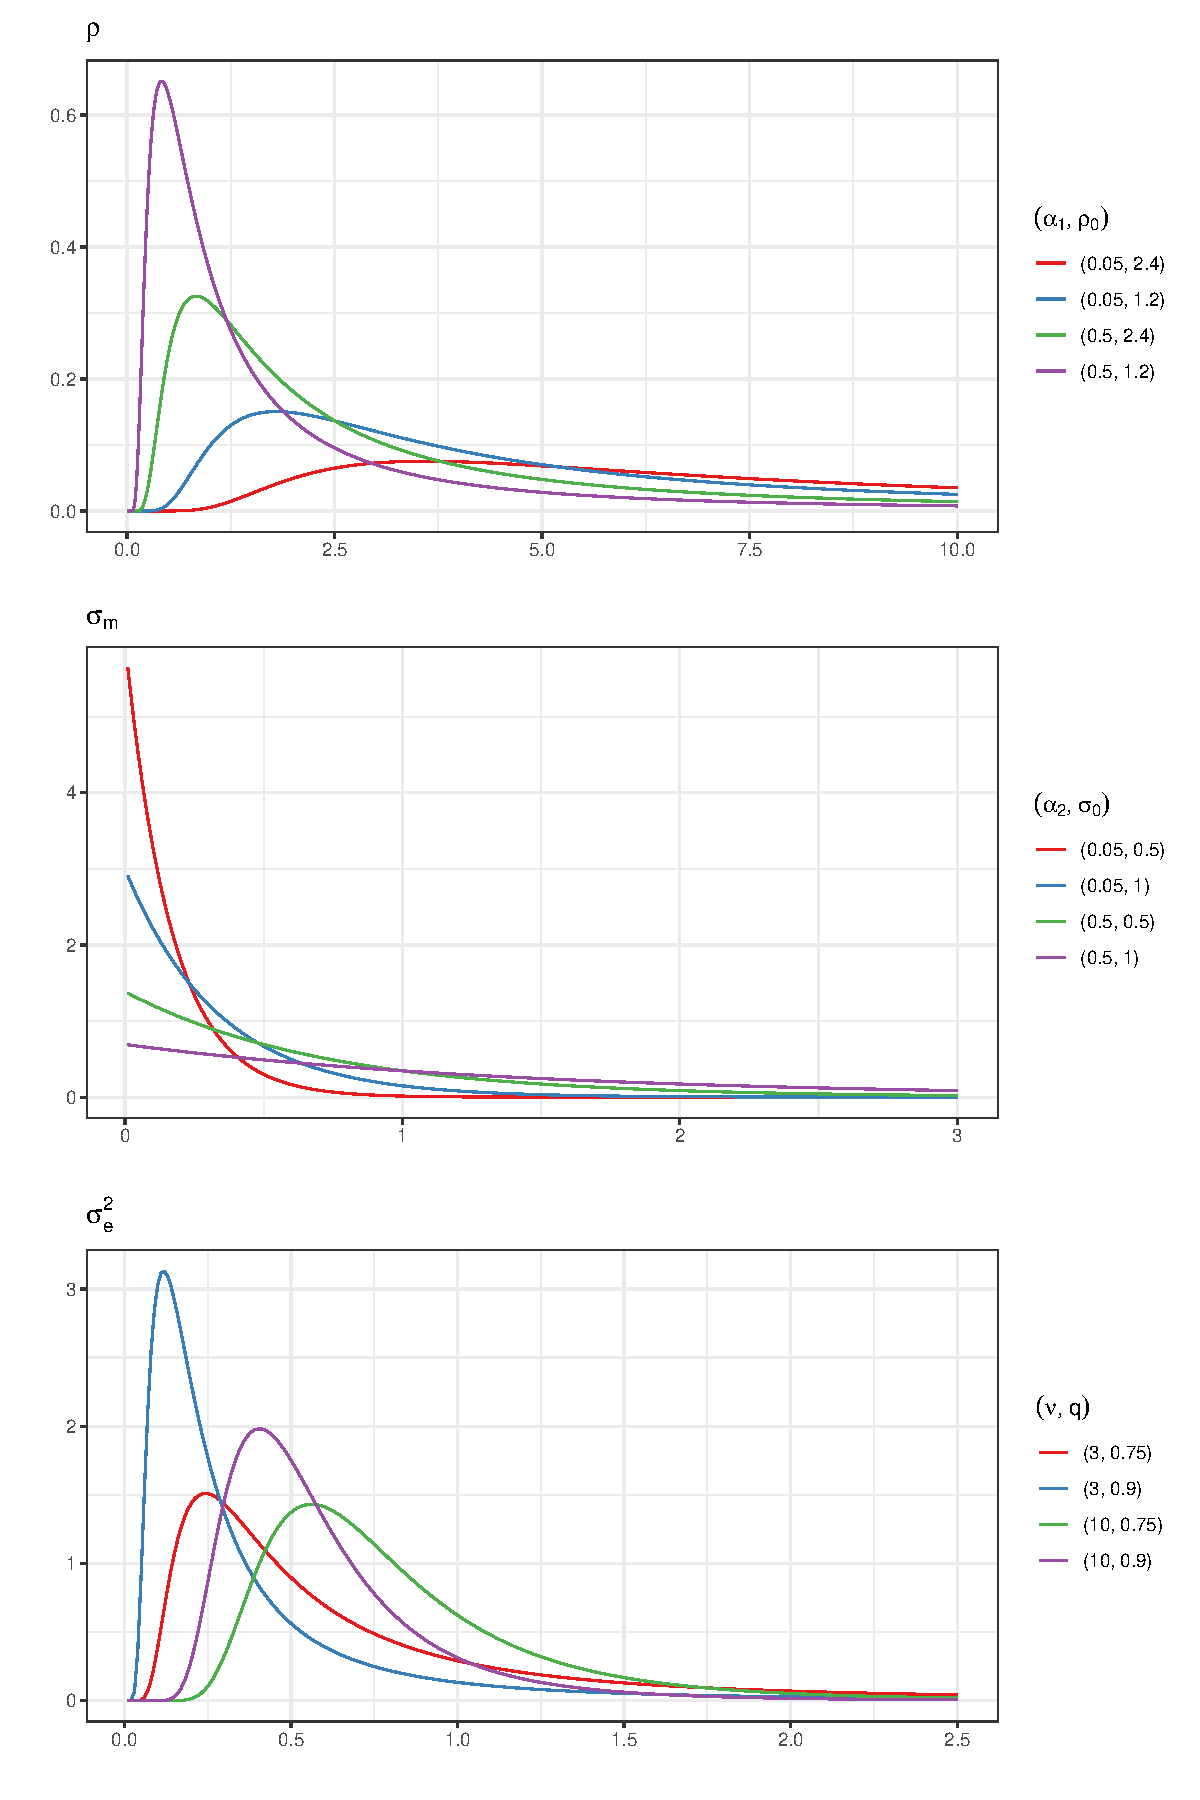
\includegraphics[width=.75\linewidth]{robustness/par_sens.pdf}
    \caption{Probability density functions of $\rho, \sigma_m$ and $\sigma_e^2$ under different values of hyperparameters. The different color labels represent different choices of hyperparameters.}
    \label{fig:robustness}
\end{figure}

\subsection{Sensitivity analysis of $\alpha_1$ and $\alpha_2$}

We consider the following four scenarios of $\alpha_1$ and $\alpha_2$: (1) $\alpha_1 = 0.5, \alpha_2 = 0.5$, (2) $\alpha_1 = 0.05, \alpha_2 = 0.5$, (3) $\alpha_1 = 0.5, \alpha_2 = 0.05$, (4) $\alpha_1 = 0.05, \alpha_2 = 0.05$. Note that scenario (1) corresponds to the default values of $\alpha_1$ and $\alpha_2$. 

\begin{table}[H]
\centering
\begin{tabular}{ccccc}
\hline
Hyperparameter Settings              & RMSE & AIS & AIL & ACR \\ \hline
${\alpha}_1 = 0.05, {\alpha}_2 = 0.05$ &
  \begin{tabular}[c]{@{}c@{}}0.0971\\ (0.0129)\end{tabular} &
  \begin{tabular}[c]{@{}c@{}}0.0148\\ (0.0046)\end{tabular} &
  \begin{tabular}[c]{@{}c@{}}0.1585\\ (0.0292)\end{tabular} &
  \begin{tabular}[c]{@{}c@{}}82.78\%\\ (0.0692)\end{tabular} \\
${\alpha}_1 = 0.05,{\alpha}_2 = 0.5$ &\begin{tabular}[c]{@{}c@{}}0.0973\\ (0.0129)\end{tabular}&
\begin{tabular}[c]{@{}c@{}}0.0149\\ (0.0046)\end{tabular}&
\begin{tabular}[c]{@{}c@{}}0.1584\\ (0.0289)\end{tabular}&
\begin{tabular}[c]{@{}c@{}}82.54\%\\ (0.0693)\end{tabular}\\
${\alpha}_1 = 0.5,{\alpha}_2 = 0.05$ &\begin{tabular}[c]{@{}c@{}}0.0975\\ (0.0130)\end{tabular}&
\begin{tabular}[c]{@{}c@{}}0.0149\\ (0.0046)\end{tabular}&
\begin{tabular}[c]{@{}c@{}}0.1584\\ (0.0291)\end{tabular}&
\begin{tabular}[c]{@{}c@{}}82.50\%\\ (0.0692)\end{tabular}\\
${\alpha}_1 = 0.5,{\alpha}_2 = 0.5$  &\begin{tabular}[c]{@{}c@{}}0.0971\\ (0.0128)\end{tabular}&
\begin{tabular}[c]{@{}c@{}}0.0147\\ (0.0044)\end{tabular}&
\begin{tabular}[c]{@{}c@{}}0.1587\\ (0.0292)\end{tabular}&
\begin{tabular}[c]{@{}c@{}}82.78\%\\ (0.0685)\end{tabular}\\ \hline
\end{tabular}
\caption{Prediction performance measures over all four scenarios of $\alpha_1$ and $\alpha_2$ combinations. The nominal coverage is 95\% and small values of AIS are preferred. The averages over $25$ test datasets are shown with standard deviations shown in brackets.}
\label{tab:sim_table}
\end{table}

\subsection{Sensitivity analysis of $\rho_0$ and $\sigma_0$}

We consider the following four scenarios of $\rho_0$ and $\sigma_0$: (1) $\rho_0 = 2.4, \sigma_0 = 0.5$, (2) $\rho_0 = 2.4, \alpha_2 = 1$, (3) $\rho_0 = 1.2, \sigma_0 = 0.5$, (4) $\rho_0 = 1.2, \sigma_0 = 1$. Note that scenario (1) corresponds to the default values of $\rho_0$ and $\sigma_0$. 

\begin{table}[H]
\centering
\begin{tabular}{ccccc}
\hline
Hyperparameter Settings              & RMSE & AIS & AIL & ACR \\ \hline
$\rho_0 = 2.4, \sigma_0 = 0.5$ &
  \begin{tabular}[c]{@{}c@{}}0.0963\\ (0.0127)\end{tabular} &
  \begin{tabular}[c]{@{}c@{}}0.0146\\ (0.0041)\end{tabular} &
  \begin{tabular}[c]{@{}c@{}}0.1580\\ (0.0255)\end{tabular} &
  \begin{tabular}[c]{@{}c@{}}82.10\%\\ (0.0580)\end{tabular} \\
$\rho_0 = 2.4, \sigma_0 = 1$ & \begin{tabular}[c]{@{}c@{}}0.0963\\ (0.0127)\end{tabular} &
\begin{tabular}[c]{@{}c@{}}0.0146\\ (0.0041)\end{tabular}&
\begin{tabular}[c]{@{}c@{}}0.1579\\ (0.0253)\end{tabular}&
\begin{tabular}[c]{@{}c@{}}82.27\%\\ (0.0596)\end{tabular}\\
$\rho_0 = 1.2, \sigma_0 = 0.5$ &\begin{tabular}[c]{@{}c@{}}0.0962\\ (0.0127)\end{tabular}&
\begin{tabular}[c]{@{}c@{}}0.0145\\ (0.0041)\end{tabular}&
\begin{tabular}[c]{@{}c@{}}0.1580\\ (0.0252)\end{tabular}&
\begin{tabular}[c]{@{}c@{}}82.35\%\\ (0.0594)\end{tabular}\\
$\rho_0 = 1.2, \sigma_0 = 1$  &\begin{tabular}[c]{@{}c@{}}0.0961\\ (0.0126)\end{tabular}&
\begin{tabular}[c]{@{}c@{}}0.0144\\ (0.0040)\end{tabular}&
\begin{tabular}[c]{@{}c@{}}0.1582\\ (0.0256)\end{tabular}&
\begin{tabular}[c]{@{}c@{}}82.61\%\\ (0.0582)\end{tabular}\\ \hline
\end{tabular}
\caption{Prediction performance measures over all four scenarios of $\rho_0$ and $\sigma_0$ combinations. The nominal coverage is 95\% and small values of AIS are preferred. The averages over $25$ test datasets are shown with standard deviations shown in brackets.}
\label{tab:sim_table}
\end{table}

\subsection{Sensitivity analysis of $\nu$ and $q$}

We consider the following four scenarios of $\nu$ and $q$: (1) $\nu = 3, q = 0.75$, (2) $\nu = 3, q = 0.9$, (3) $\nu = 10, q = 0.75$, (4) $\nu = 10, q = 0.9$. Note that scenario (1) corresponds to the default values of $\nu$ and $q$. 

\begin{table}[!h]
\centering
\begin{tabular}{ccccc}
\hline
Hyperparameter Settings              & RMSE & AIS & AIL & ACR \\ \hline
$\nu = 3, q = 0.75$ &
  \begin{tabular}[c]{@{}c@{}}0.0988\\ (0.0135)\end{tabular} &
  \begin{tabular}[c]{@{}c@{}}0.0152\\ (0.0044)\end{tabular} &
  \begin{tabular}[c]{@{}c@{}}0.1590\\ (0.0248)\end{tabular} &
  \begin{tabular}[c]{@{}c@{}}82.21\%\\ (0.0615)\end{tabular} \\
$\nu = 3, q = 0.9$ &\begin{tabular}[c]{@{}c@{}}0.0961\\ (0.0127)\end{tabular}&
\begin{tabular}[c]{@{}c@{}}0.0145\\ (0.0041)\end{tabular}&
\begin{tabular}[c]{@{}c@{}}0.1580\\ (0.0252)\end{tabular}&
\begin{tabular}[c]{@{}c@{}}82.48\%\\ (0.0589)\end{tabular}\\
$\nu = 10, q = 0.75$ &\begin{tabular}[c]{@{}c@{}}0.0967\\ (0.0129)\end{tabular}&
\begin{tabular}[c]{@{}c@{}}0.0146\\ (0.0039)\end{tabular}&
\begin{tabular}[c]{@{}c@{}}0.1597\\ (0.0232)\end{tabular}&
\begin{tabular}[c]{@{}c@{}}83.15\%\\ (0.0523)\end{tabular}\\
$\nu = 10, q = 0.9$  &\begin{tabular}[c]{@{}c@{}}0.0964\\ (0.0148)\end{tabular}&
\begin{tabular}[c]{@{}c@{}}0.0147\\ (0.0044)\end{tabular}&
\begin{tabular}[c]{@{}c@{}}0.1577\\ (0.0236)\end{tabular}&
\begin{tabular}[c]{@{}c@{}}82.23\%\\ (0.0581)\end{tabular}\\ \hline
\end{tabular}
\caption{Prediction performance measures over all four scenarios of $\nu$ and $q$ combinations. The nominal coverage is 95\% and small values of AIS are preferred. The averages over $25$ test datasets are shown with standard deviations shown in brackets.}
\label{tab:sim_table}
\end{table}


\newpage




\section{Additional results from discussion on the robustness of BARTSIMP}

\begin{figure}[H]
    \centering
    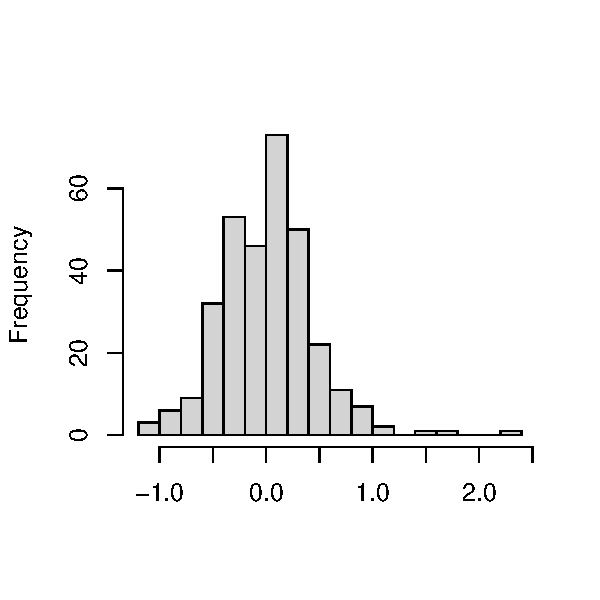
\includegraphics[width=0.5\linewidth]{robustness/hist.pdf}
    \caption{Histogram of the residual values from the BARTSIMP model fit to the WHZ application example.}
    \label{fig:robust1}
\end{figure}

\begin{figure}[H]
    \centering
    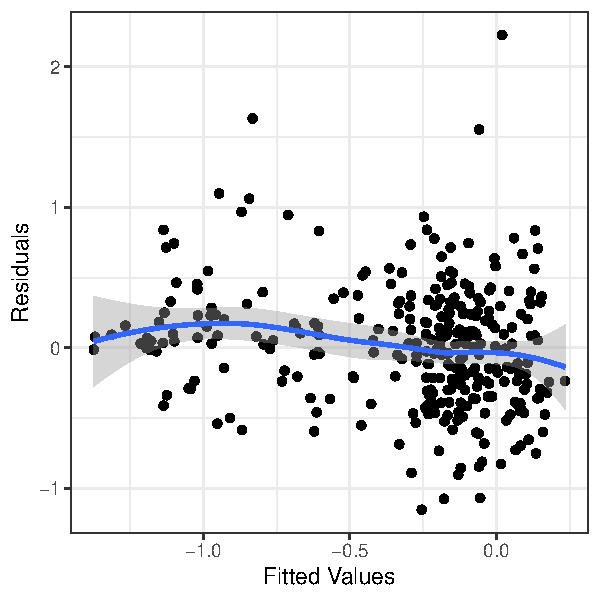
\includegraphics[width=0.5\linewidth]{robustness/smooth.pdf}
    \caption{Scatterplot of the residual values (y-axis) and the fitted values (x-axis) from the BARTSIMP model fit to the WHZ application example.}
    \label{fig:robust2}
\end{figure}

\section{Admin 2 Results for the Application Example}

Figures \ref{fig:admin2areas_med} and \ref{fig:admin2areas_cw} show maps of posterior median and 95\% credible interval lengths for the four methods: BARTSIMP, BART, SPDE and SPDE0. Note that the results are similar to the results for Admin 1 areas, where the point predictions are similar across different methods, while BARTSIMP has larger confidence interval lengths than all other methods. Figures \ref{fig:admin2areas_intervals1} to \ref{fig:admin2areas_intervals6} plots the posterior median and 95\% credible intervals for all 290 Admin 2 enumeration areas. Note that we have split the graphs into six sub-graphs due to the amount of Admin 2 areas in consideration. 

\begin{figure}[H]
\centering
\includegraphics[width = \linewidth]{admin2_areal_med.pdf}
\caption{Maps of Admin 2 level WHZ posterior median (left) and 95\% credible interval lengths (right) for BARTSIMP, BART, SPDE and SPDE0.}
\label{fig:admin2areas_med}
\end{figure}

\begin{figure}[H]
\centering
\includegraphics[width = \linewidth]{admin2_areal_cw.pdf}
\caption{Maps of Admin 2 level WHZ posterior median (left) and 95\% credible interval lengths (right) for BARTSIMP, BART, SPDE and SPDE0.}
\label{fig:admin2areas_cw}
\end{figure}

\begin{figure}[H]
\centering
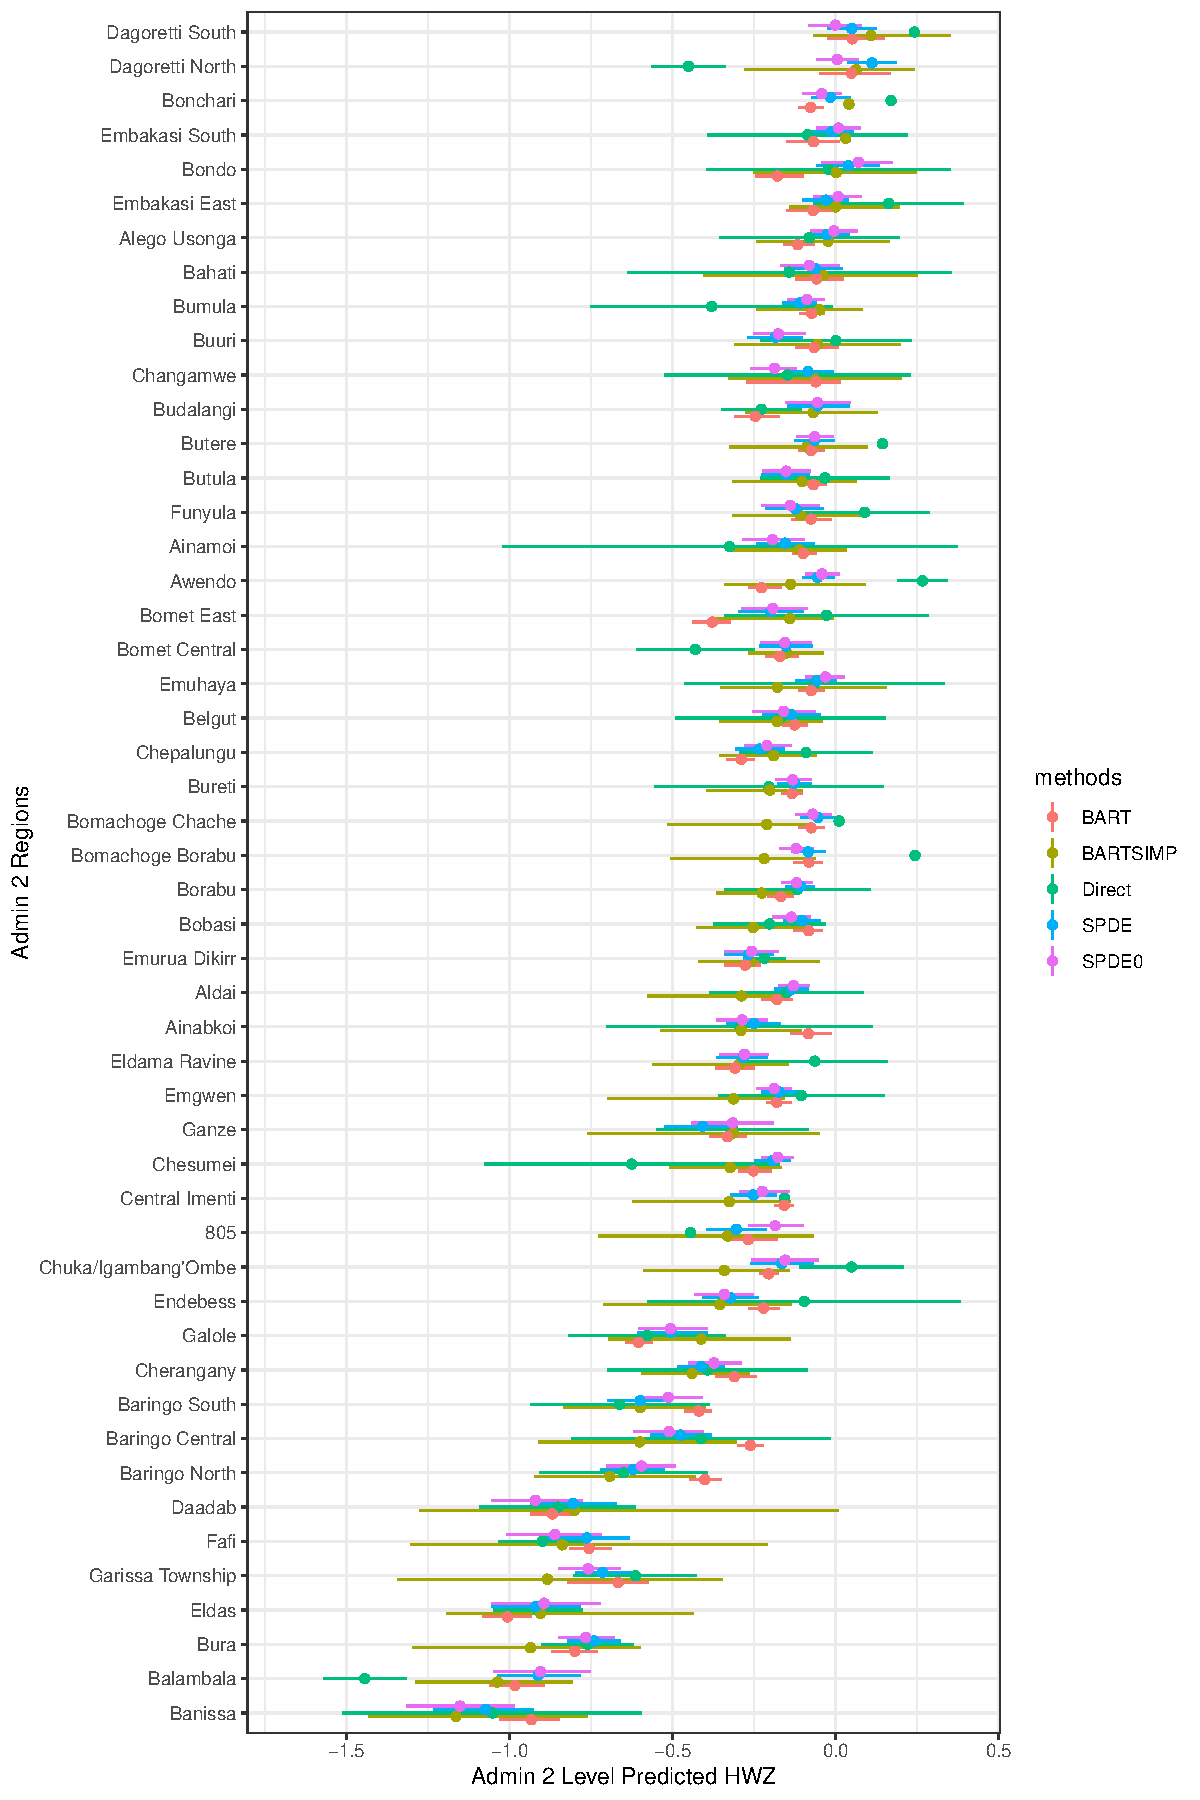
\includegraphics[width = .8\linewidth]{admin2_agg/admin2_aggregated_comparisons_p1.pdf}
\caption{The Admin 2 level posterior median and 95\% credible/confidence intervals of
WHZ for BART, BARTSIMP, SPDE0, SPDE and direct (weighted) estimates. The Admin
1 areas are arranged according to the predicted posterior mean given by BARTSIMP.}
\label{fig:admin2areas_intervals1}
\end{figure}

\begin{figure}[H]
\centering
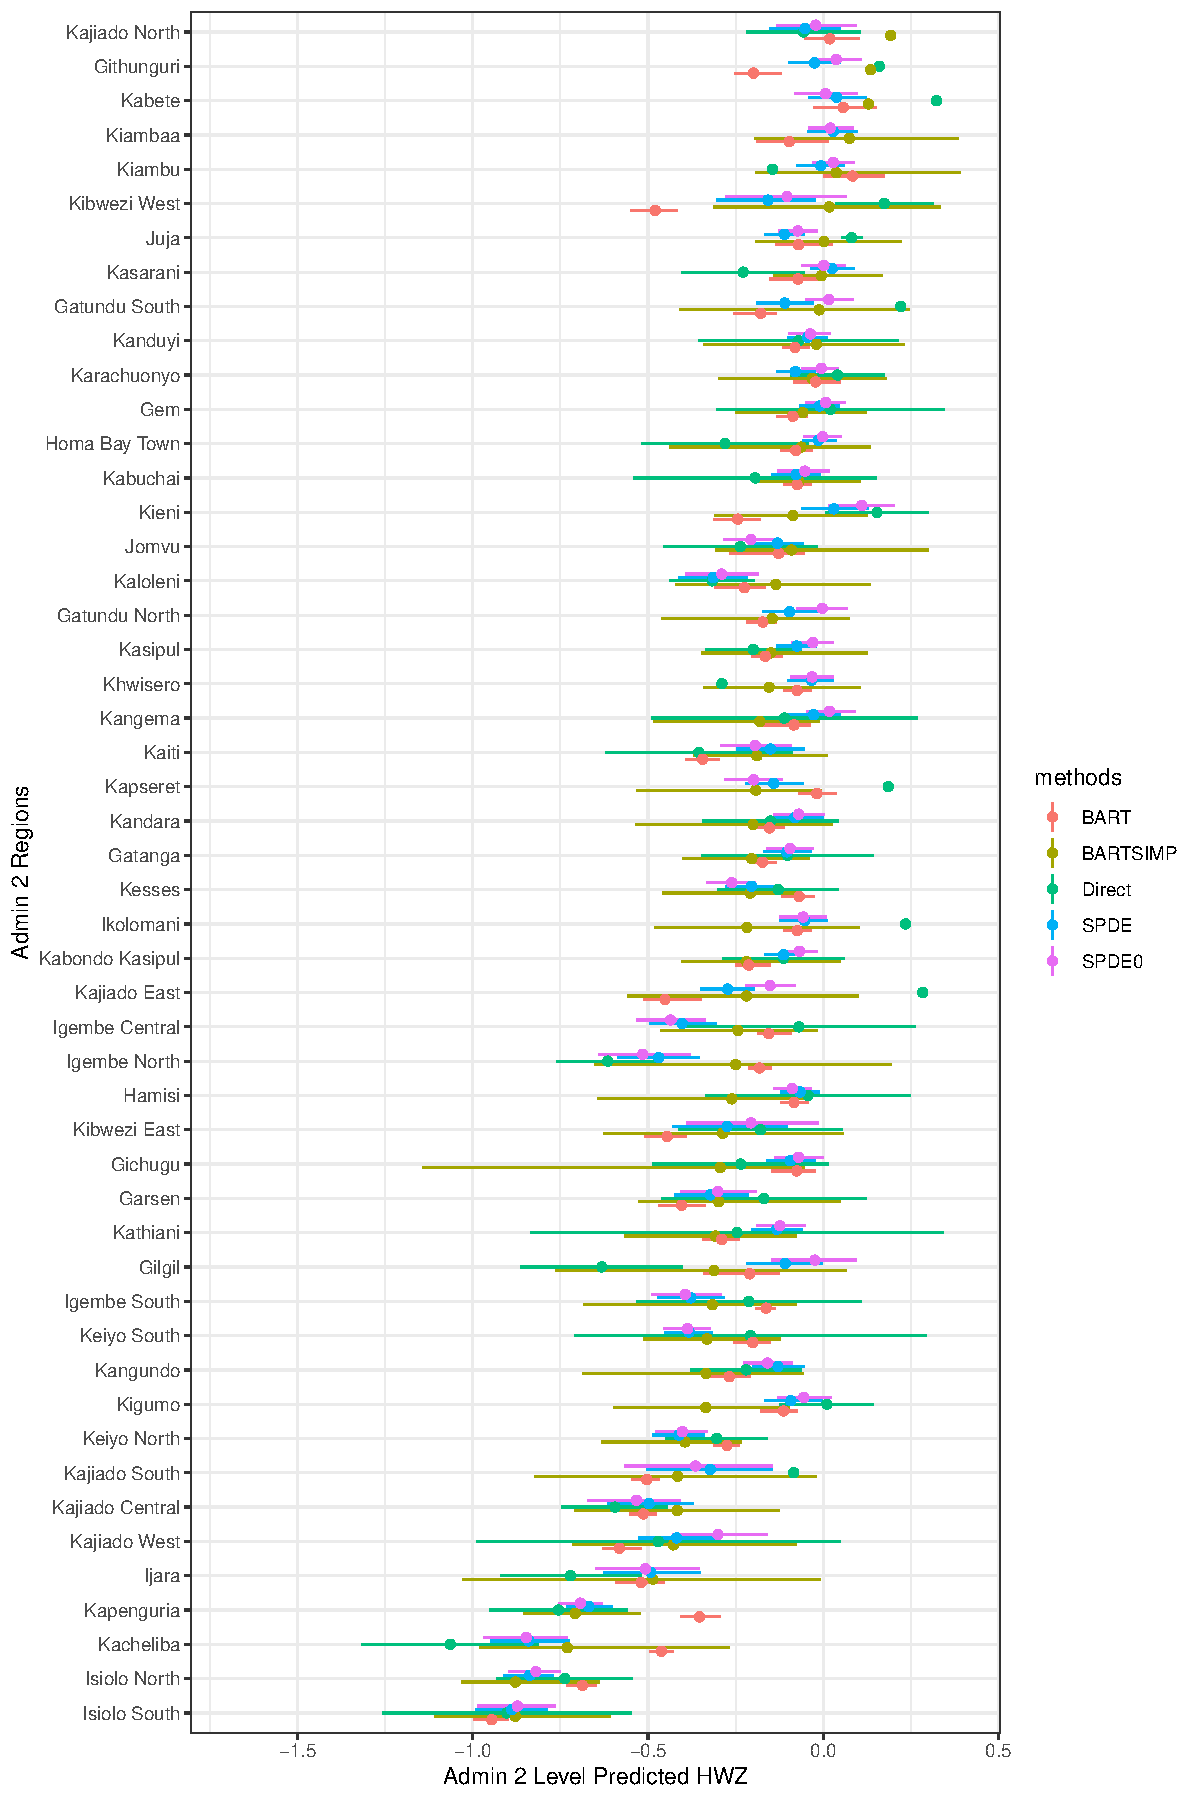
\includegraphics[width = .8\linewidth]{admin2_agg/admin2_aggregated_comparisons_p2.pdf}
\caption{The Admin 2 level posterior median and 95\% credible/confidence intervals of
WHZ for BART, BARTSIMP, SPDE0, SPDE and direct (weighted) estimates. The Admin
1 areas are arranged according to the predicted posterior mean given by BARTSIMP.}
\label{fig:admin2areas_intervals2}
\end{figure}

\begin{figure}[H]
\centering
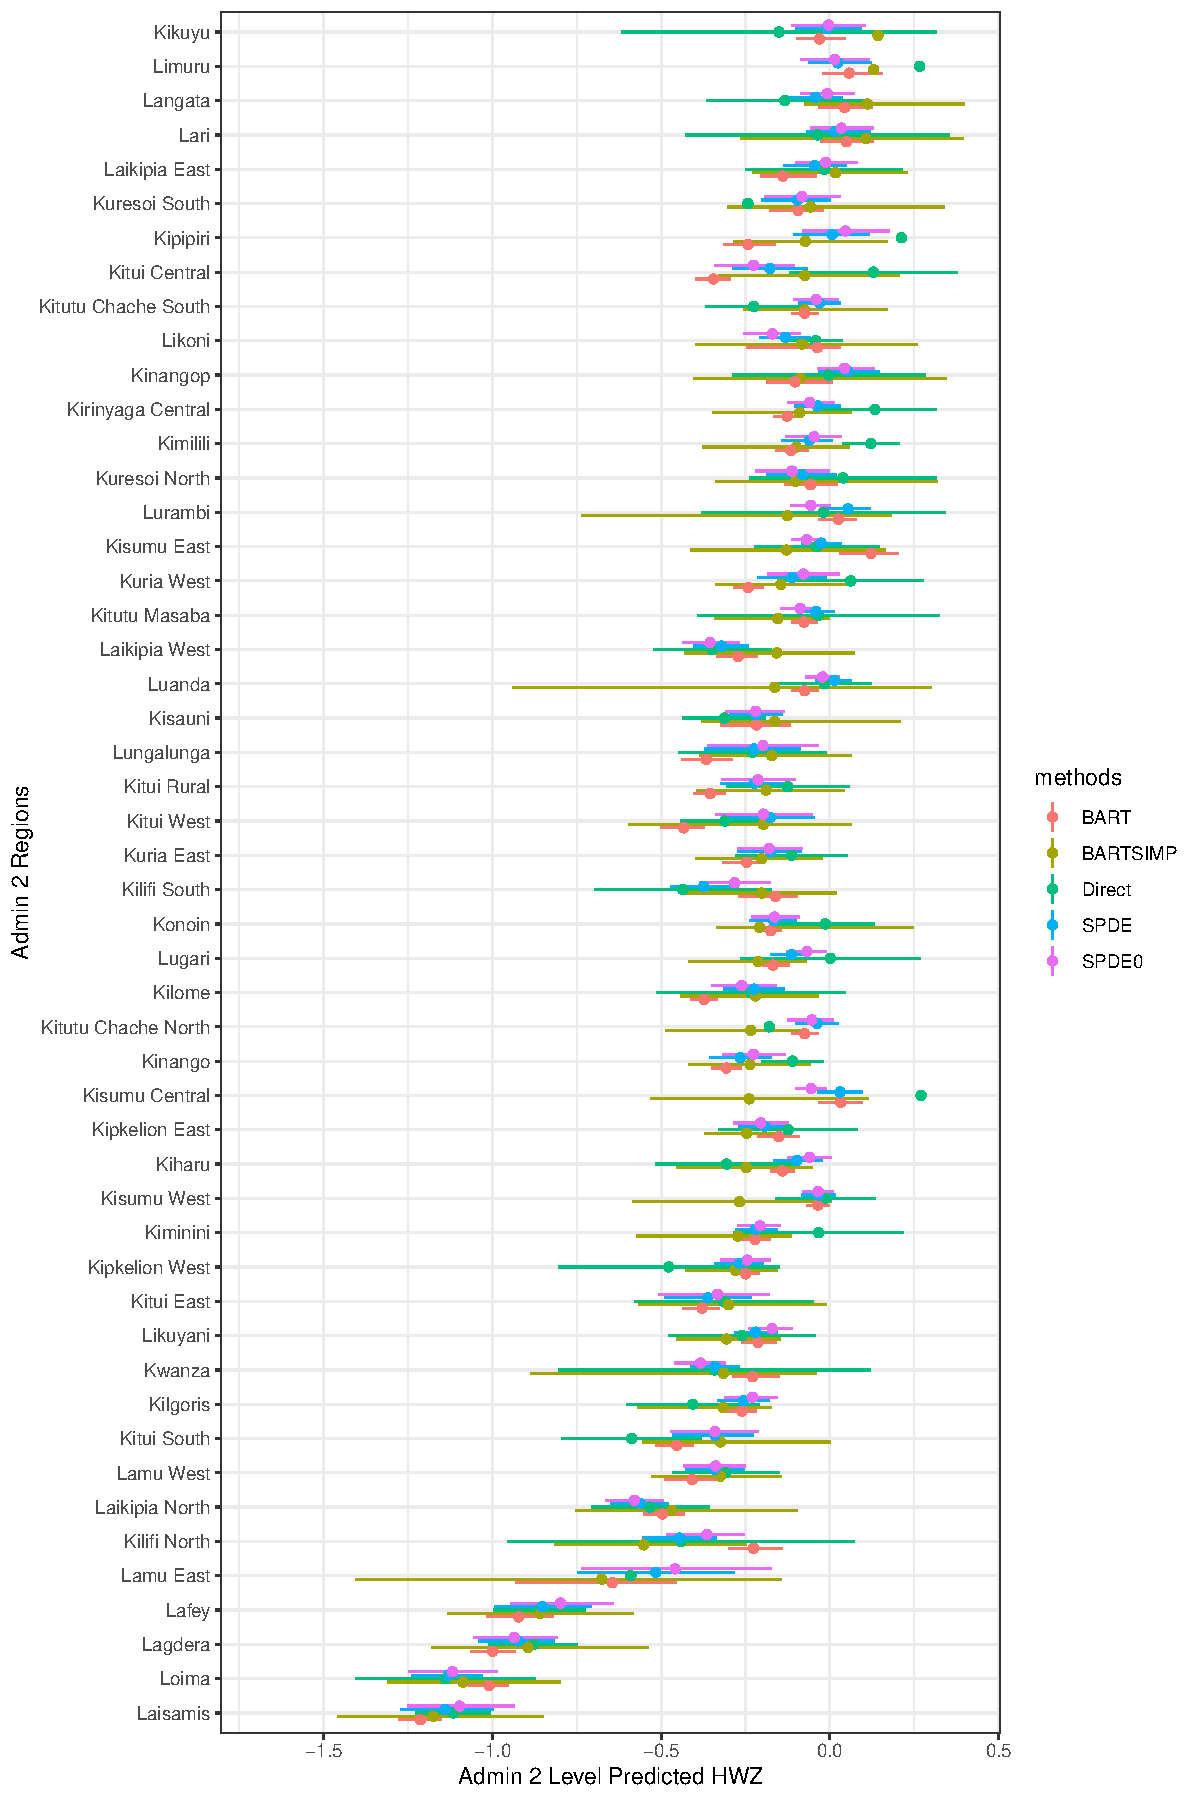
\includegraphics[width = .8\linewidth]{admin2_agg/admin2_aggregated_comparisons_p3.pdf}
\caption{The Admin 2 level posterior median and 95\% credible/confidence intervals of
WHZ for BART, BARTSIMP, SPDE0, SPDE and direct (weighted) estimates. The Admin
1 areas are arranged according to the predicted posterior mean given by BARTSIMP.}
\label{fig:admin2areas_intervals3}
\end{figure}

\begin{figure}[H]
\centering
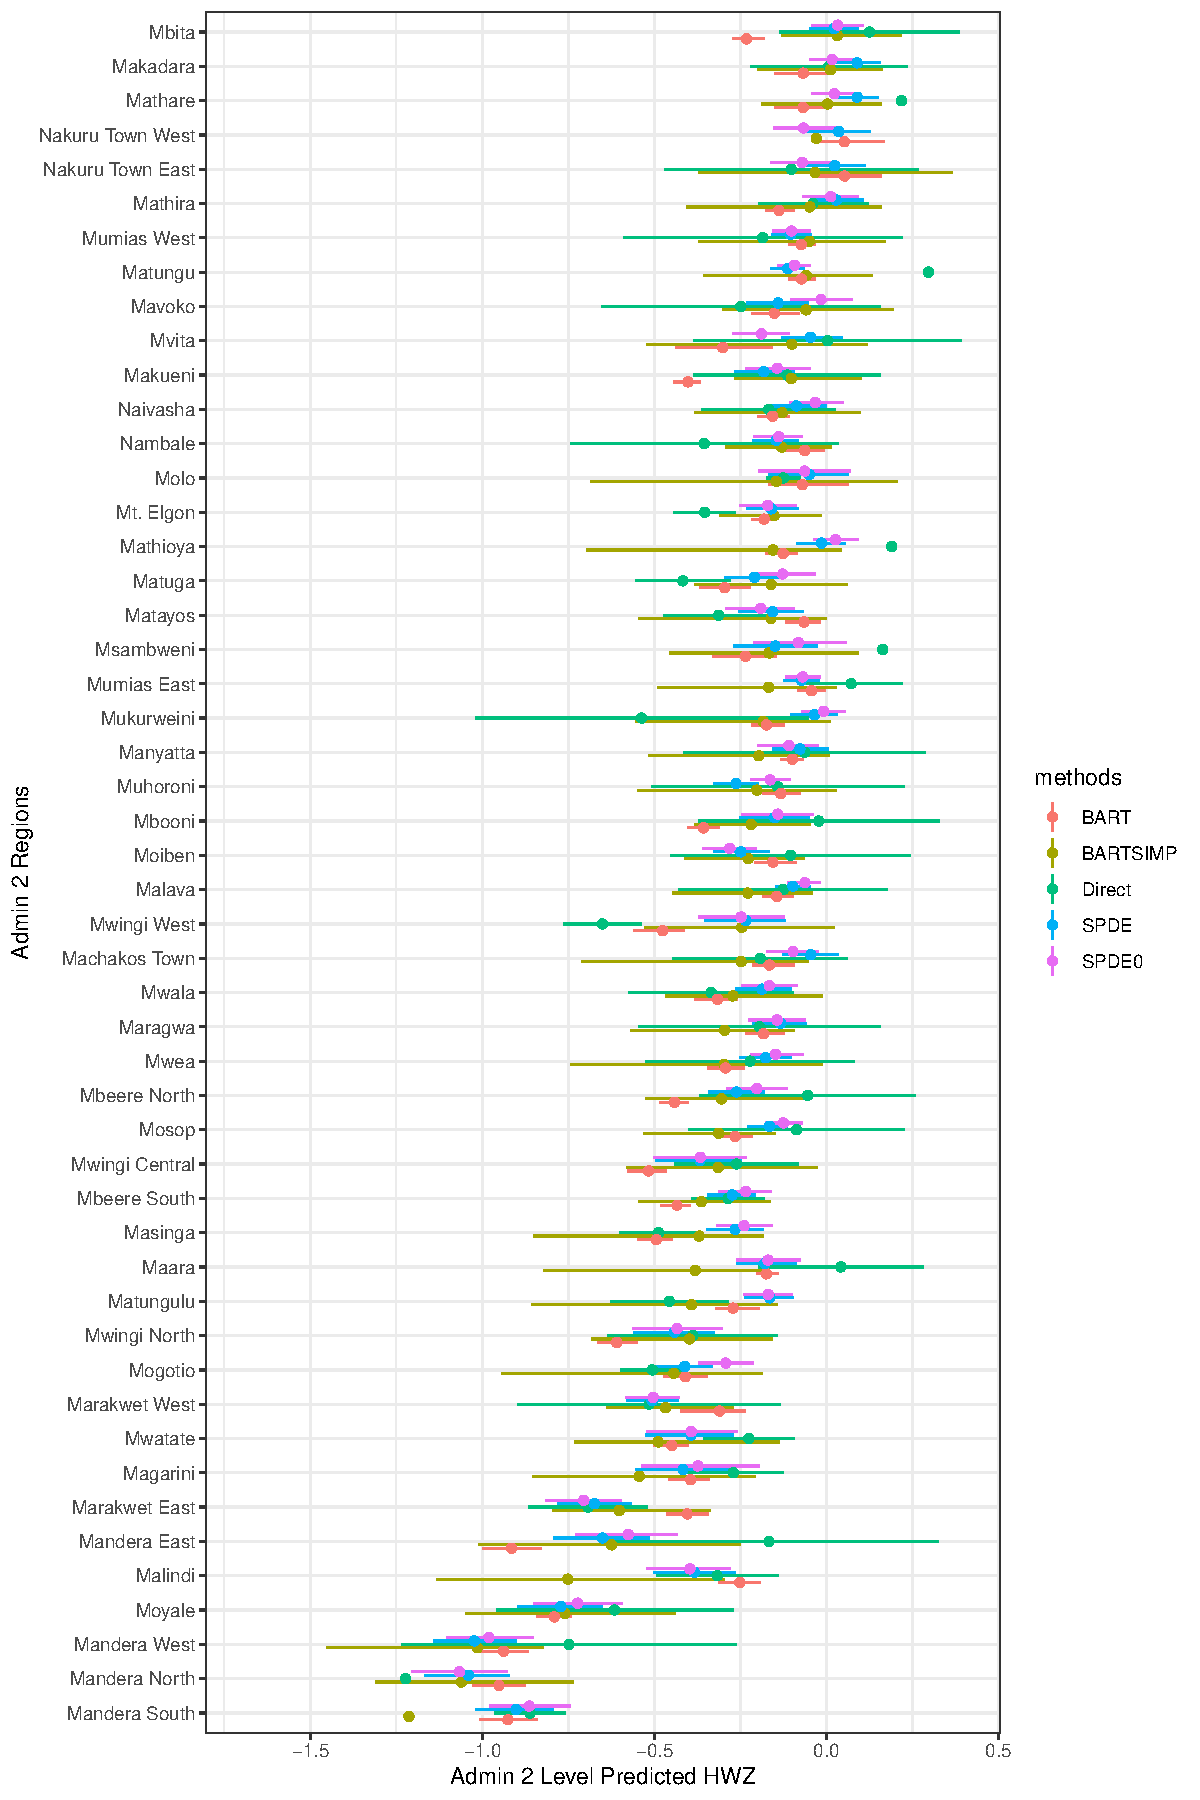
\includegraphics[width = .8\linewidth]{admin2_agg/admin2_aggregated_comparisons_p4.pdf}
\caption{The Admin 2 level posterior median and 95\% credible/confidence intervals of
WHZ for BART, BARTSIMP, SPDE0, SPDE and direct (weighted) estimates. The Admin
1 areas are arranged according to the predicted posterior mean given by BARTSIMP.}
\label{fig:admin2areas_intervals4}
\end{figure}

\begin{figure}[H]
\centering
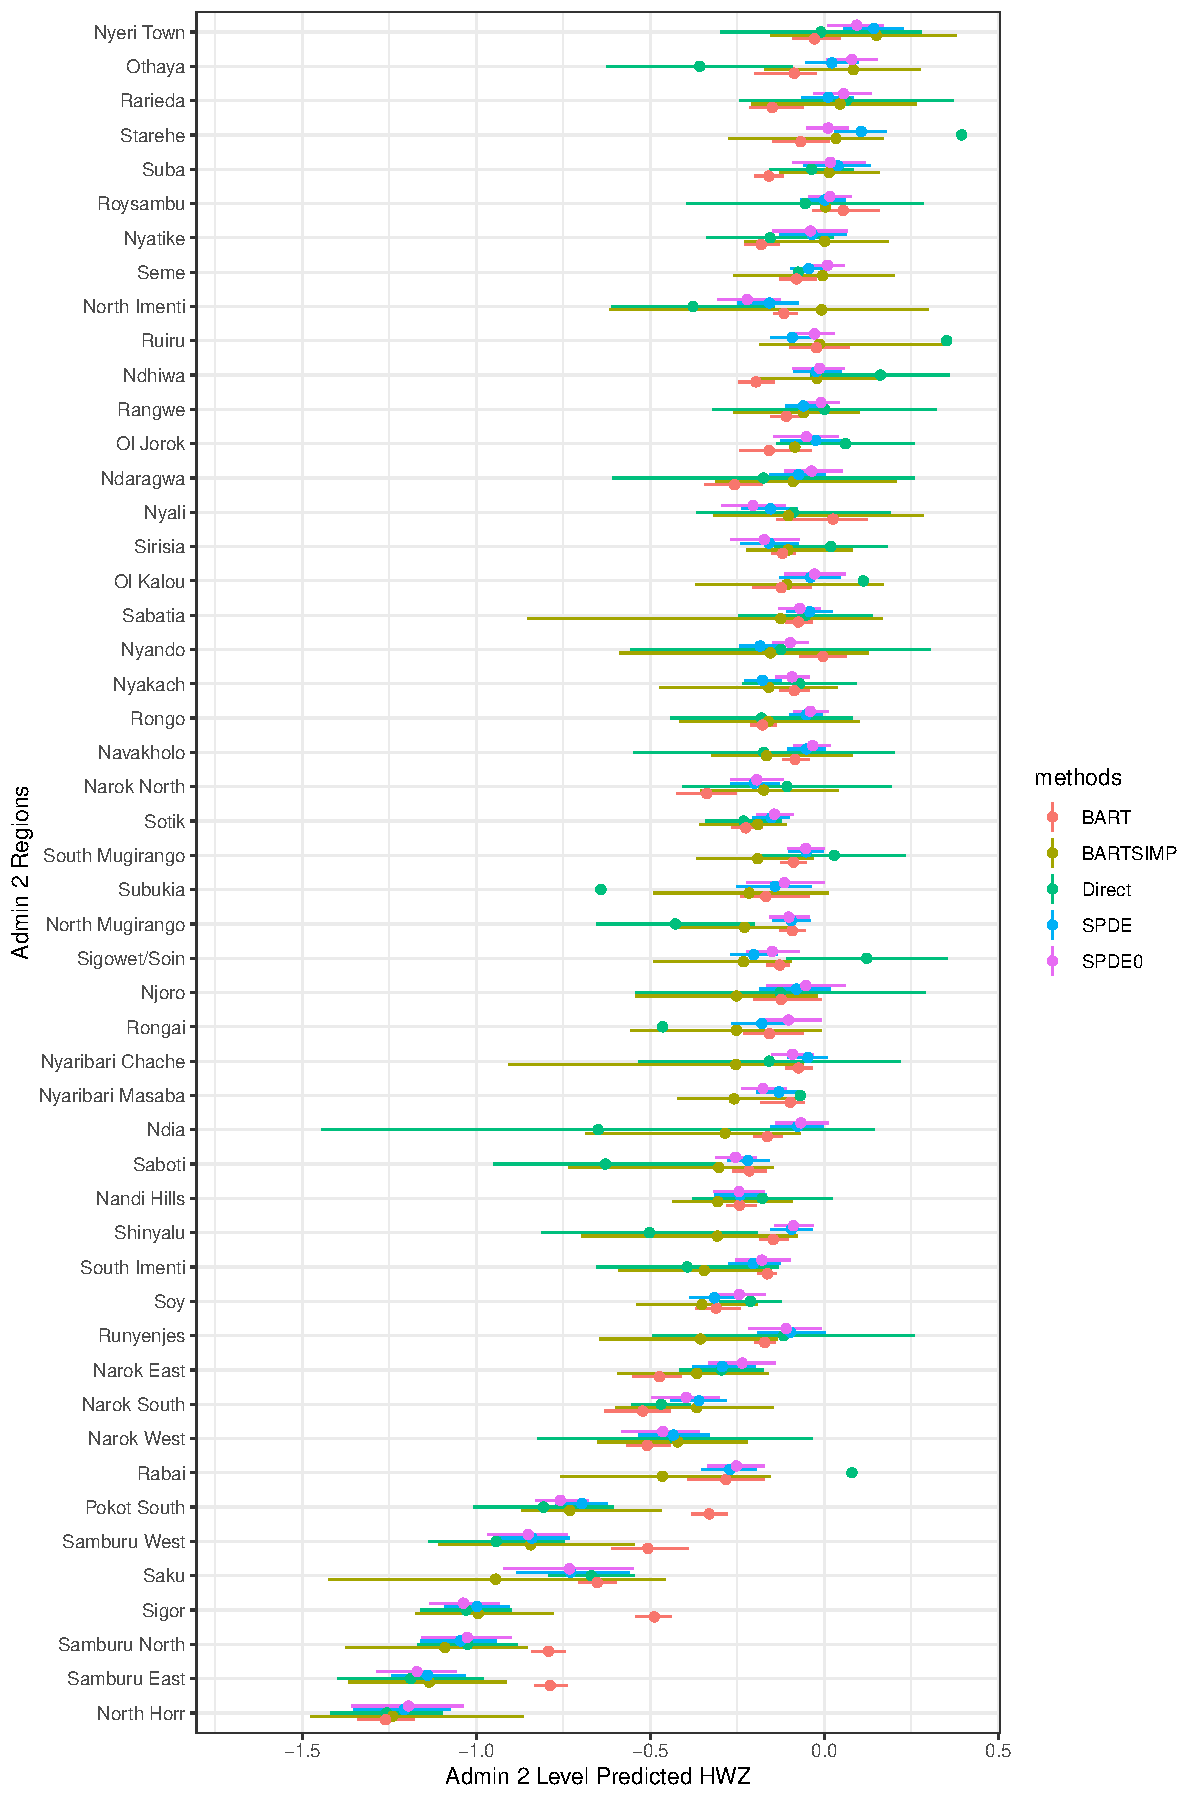
\includegraphics[width = .8\linewidth]{admin2_agg/admin2_aggregated_comparisons_p5.pdf}
\caption{The Admin 2 level posterior median and 95\% credible/confidence intervals of
WHZ for BART, BARTSIMP, SPDE0, SPDE and direct (weighted) estimates. The Admin
1 areas are arranged according to the predicted posterior mean given by BARTSIMP.}
\label{fig:admin2areas_intervals5}
\end{figure}

\begin{figure}[H]
\centering
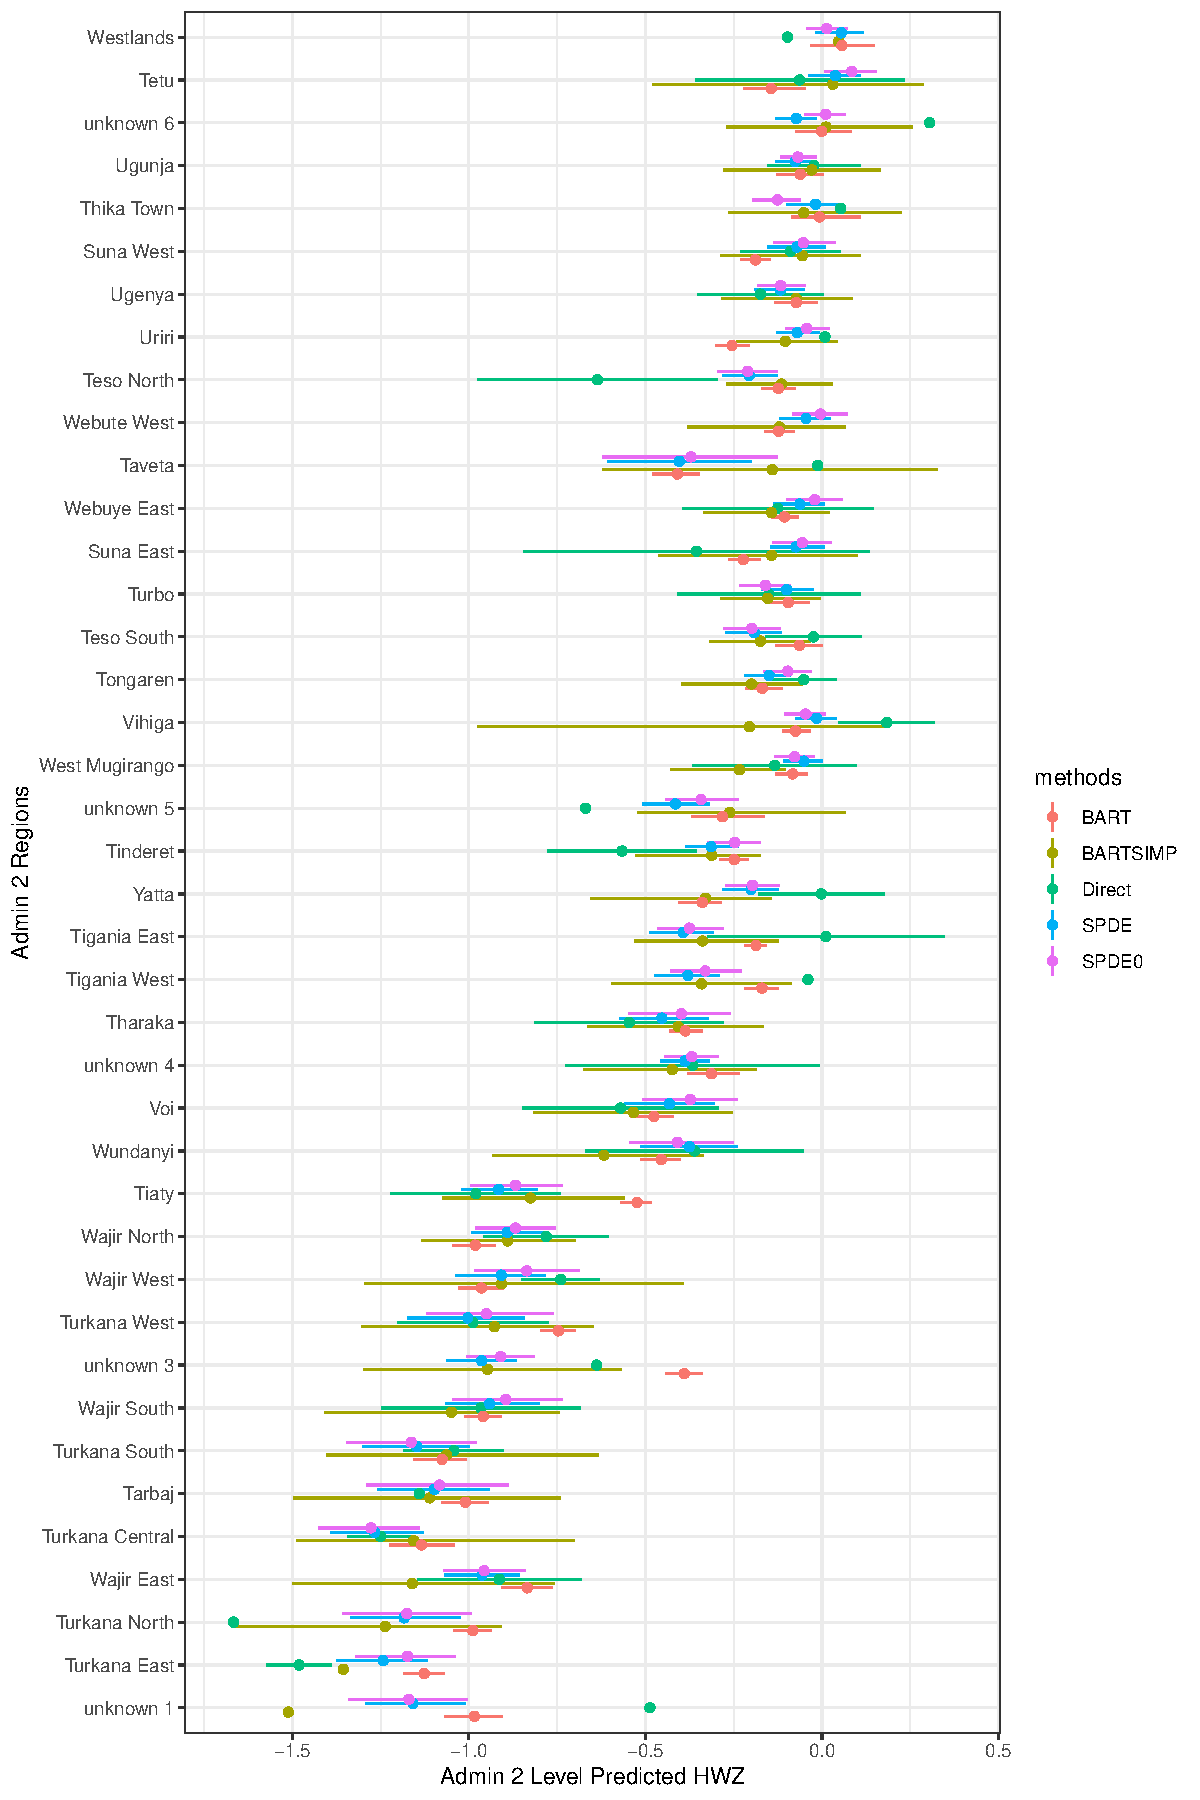
\includegraphics[width = .8\linewidth]{admin2_agg/admin2_aggregated_comparisons_p6.pdf}
\caption{The Admin 2 level posterior median and 95\% credible/confidence intervals of
WHZ for BART, BARTSIMP, SPDE0, SPDE and direct (weighted) estimates. The Admin
1 areas are arranged according to the predicted posterior mean given by BARTSIMP.}
\label{fig:admin2areas_intervals6}
\end{figure}

\newpage




\section{Addition Information on DHS Geospatial Covariates Used in the Model}

See towards the end of the document.

\begin{sidewaystable}[tb]
\small
\centering
\caption{DHS Geospatial covariates used in our model.\\}
\begin{tabular}{lllccc}
\hline
\textbf{Variable} &
  \textbf{Years} &
  \textbf{Source} &
  \textbf{Original Range} &
  \textbf{Transformed Range} &
  \textbf{Transformation} \\
\hline
Population Density &
  2014 &
  \begin{tabular}[c]{@{}c@{}}WorldPop\tablefootnote{http://www.worldpop.org.uk/data/get\_data/. Unit is number of people per pixel.} \end{tabular} & (0.113, 116.909)
  & (-1.543, 4.762) & $\log(x + 0.1)$ \\
\hline
Night Time Light &
  2013 &
  \begin{tabular}[l]{@{}l@{}}National Centers for\\ Environmental Information\tablefootnote{https://ngdc.noaa.gov/eog/dmsp/downloadV4composites.html.} \end{tabular} & (0.001, 6.300)
  & (-0.693, 4.151) & $\log(x + 0.5)$ \\
\hline
Vegetation Index &
  2013--2014 &
  \begin{tabular}[l]{@{}l@{}}NASA EOSDIS Land Processes\\ DAAC\tablefootnote{https://lpdaac.usgs.gov/dataset\_discovery/modis/modis\_products\_table/mod13a3\_v006.} \end{tabular} & (-1.744, 2.974)
  & (-1.744, 2.974) & $x$ \\
\hline
Average Temperature &
  \begin{tabular}[l]{@{}l@{}}Mean value over\\ the period\\ 1970--2000\end{tabular} &
  \begin{tabular}[c]{@{}c@{}}WorldClim\tablefootnote{http://worldclim.org/version2. Unit is in Celsius temperature (recentered).} \end{tabular} &
 (-3.490,1.432)  & (-3.490,1.432) & $x$ \\
\hline
Precipitation &
  \begin{tabular}[l]{@{}l@{}}Mean value over\\ the period\\ 1970--2000\end{tabular} &
  \begin{tabular}[c]{@{}l@{}}WorldClim\tablefootnote{http://worldclim.org/version2. Unit: in millimeters.} \end{tabular} &
 (0.060, 22.187) & (-1.835, 3.104) & $\log(x + 0.1)$ \\
\hline
Access to Nearest City &
  2000 &
  \begin{tabular}[l]{@{}l@{}}Joint Research Centre of the\\ European Commission\tablefootnote{http://forobs.jrc.ec.europa.eu/products/gam/download.php. Measured in travel time.} \end{tabular} & (0.001, 5.633)
  & (-8.862, 1.728) & $\log x $\\
\hline
\end{tabular}
\label{tab:cov}
\end{sidewaystable}


\section{Partial Dependence Plot on the Transformed Scale}

The partial dependence plot for all six geospatial covariates is shown in Figure 5 on the paper. Due to the log-transformation we applied to a few of the covariates, the partial dependence plots on some of the covariates are gridded unevenly. As an alternative, we also included an alternative version of the partial dependence plots in Figure 12, Supplementary Materials Section 5, with $x$ on the transformed scale. Please refer to Table 1 (in the Supplementary Materials) for detailed information on the scales of the variables, before and after transformation. 

\begin{figure}[H]
    \centering
    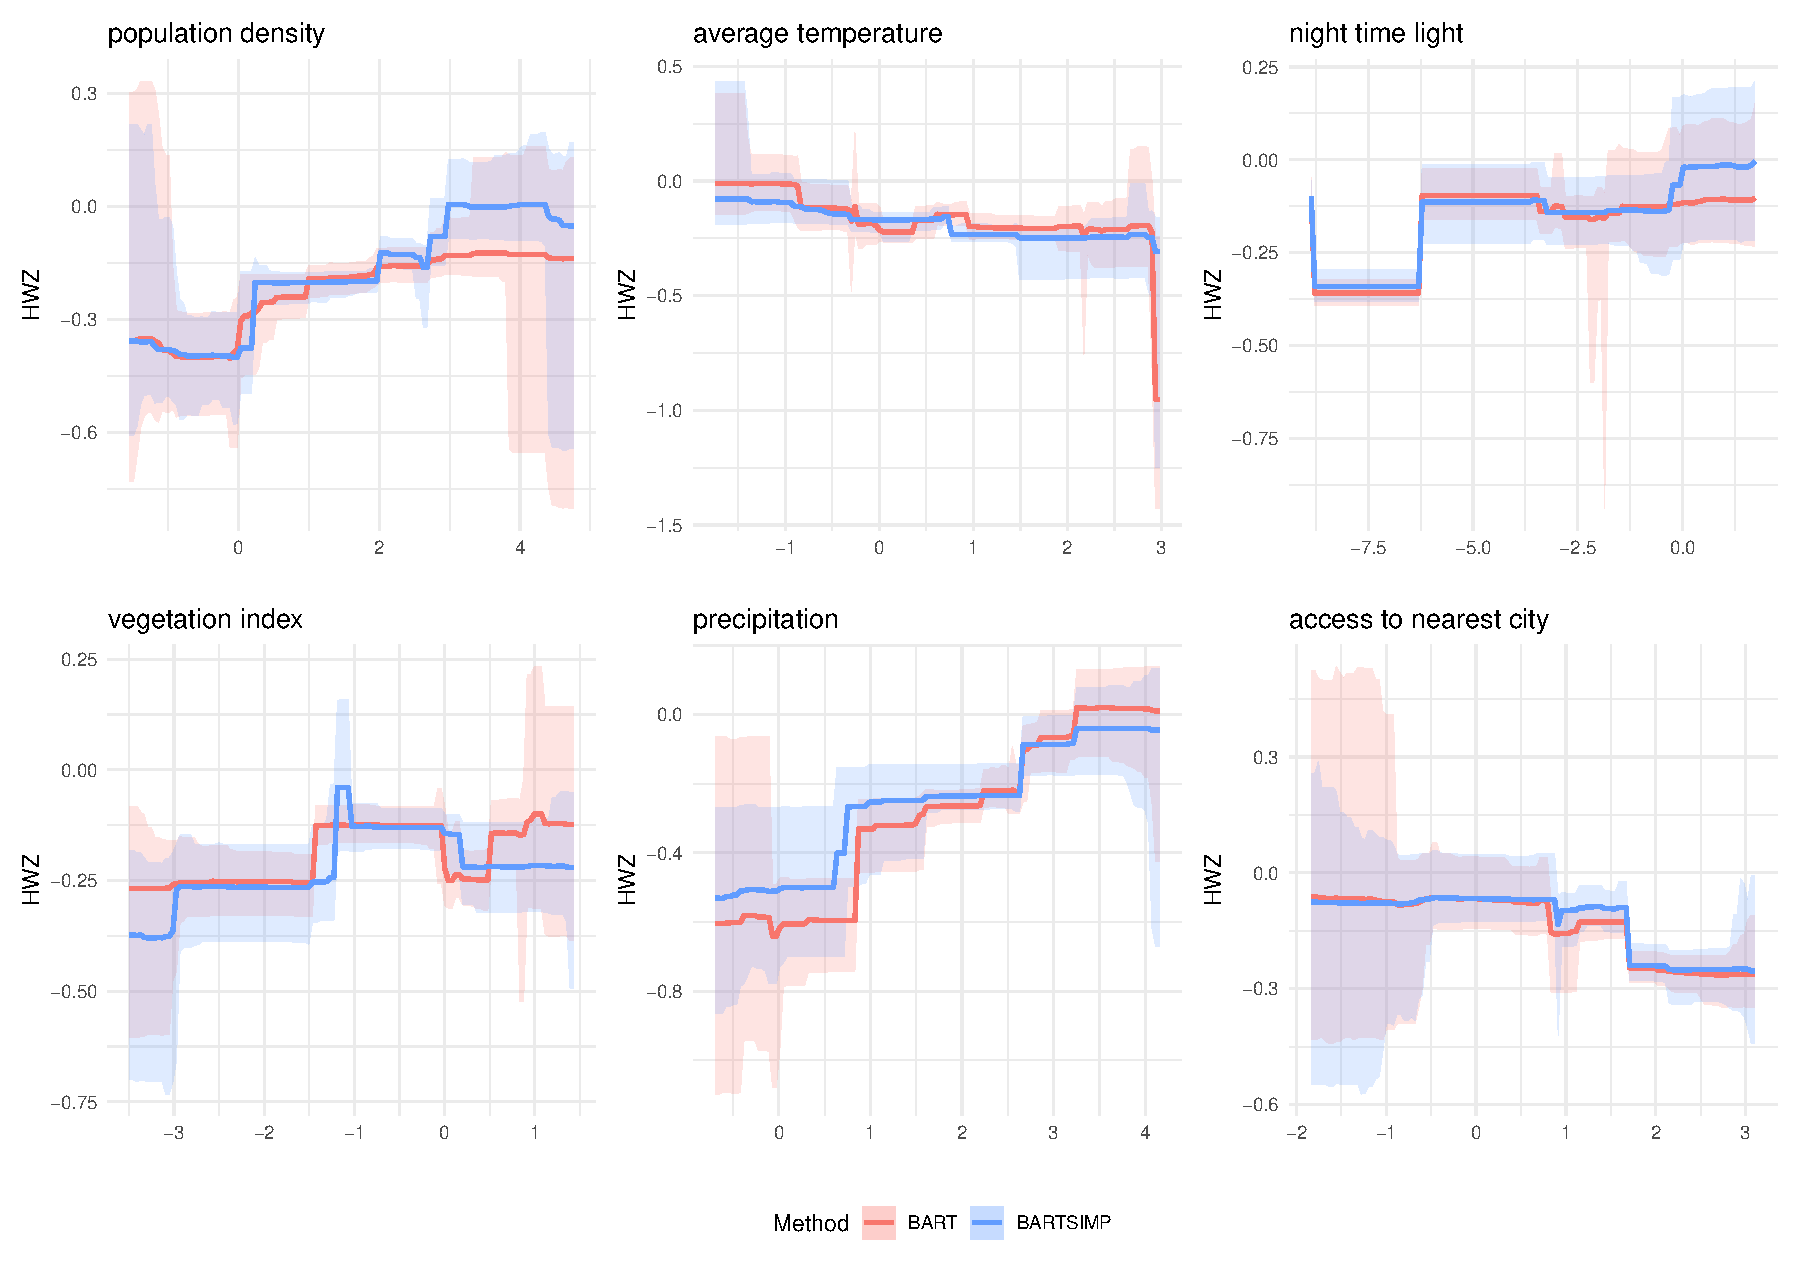
\includegraphics[width=\linewidth]{partial/res.pdf}
    \caption{Partial dependence function for all six covariates (population density on the transformed scaled, average
temperature, night time light, vegetation index, precipitation and access to nearest city)
and the 95\% pointwise credible interval provided by the BARTSIMP (blue) and BART
(red) methods.}
    \label{fig:enter-label}
\end{figure}

\newpage

\section{Spatial Results}

Figure \ref{tab:spat} shows posterior summary of the fixed effects in the SPDE model we fitted for the WHZ dataset. Note that in the table, the population density is positively significant, while covariates including vegetation index and access to nearest city, average temperature are negatively significant. This matches with the results in the partial dependence plot (see Figure 7 in the main paper). 

\begin{table}[H]
\label{tab:spat}
\centering
\begin{tabular}{rrrrr}
  \hline
 & Posterior Mean & 2.5 Percentile & Median & 97.5 Percentile \\ 
  \hline
(Intercept) & -0.61 & -0.82 & -0.62 & -0.30 \\ 
 population density & 0.06 & 0.03 & 0.06 & 0.09 \\ 
  vegetation index & -0.01 & -0.05 & -0.01 & 0.02 \\ 
  access to nearest city & -0.03 & -0.05 & -0.03 & -0.01 \\ 
  average temperature  & -0.12 & -0.18 & -0.12 & -0.06 \\ 
  night time light & 0.01 & -0.01 & 0.01 & 0.03 \\ 
  precipitation & 0.02 & -0.05 & 0.02 & 0.10 \\ 
   \hline
\end{tabular}
\caption{Posterior summary of the fixed effects in the SPDE model.}
\end{table}

\newpage

\section{Algorithmic Details on BARTSIMP}

We next provide an overview of the Metropolis-within-Gibbs algorithm we will be using for the BARTSIMP model, where the INLA-within-MCMC approach is applied to approximate the acceptance ratio.  We let $T_{-j}, \boldsymbol{\mu}_{-j}$  be the set of trees and terminal node values, respectively, not including $T_j$ and $\boldsymbol{\mu}_j$. An outline of the MCMC routine is given in Algorithm \ref{algo:bartsimp}. We now describe each of the updates.
\begin{algorithm}[!htb]
\SetAlgoLined
\textbf{Input:} Initialized values for $\mathbf{T}, \boldsymbol{\mu}, \sigma_e^2, \psi$ for a number of MCMC iterations $B$. \\
\For{$b \gets 1$ \KwTo $B$}{
\For{$j \gets 1$ \KwTo $m$}{
  \textbf{Update} $T_j \mid \boldsymbol{y}, T_{-j}, \boldsymbol{\mu}_{-j}, \sigma_e^2, \boldsymbol{\psi}$. \\ %using Bayesian-backfitting and INLA-within-MCMC algorithm. \\
  \textbf{Update} $\boldsymbol{\mu}_j \mid \boldsymbol{y}, T_j, T_{-j}, \boldsymbol{\mu}_{-j}, \sigma_e^2, \boldsymbol{\psi}$. \\ %through a Gibbs update algorithm.
  \textbf{Update} $\sigma_e^2 \mid \boldsymbol{y}, \mathbf{T}, \boldsymbol{\mu}, \boldsymbol{\psi}$. \\ % using INLA-within-MCMC. \\
  \textbf{Update} $\boldsymbol{\psi} \mid \boldsymbol{y}, \mathbf{T}, \boldsymbol{\mu}, \sigma_e^2$. \\ % using INLA-within-MCMC.
  }
}
 \caption{An overview of the BARTSIMP algorithm.}
 \label{algo:bartsimp}
\end{algorithm}\\

\subsection{Update \texorpdfstring{$T_j \mid \boldsymbol{y}, T_{-j}, \boldsymbol{\mu}_{-j}, \sigma_e^2, \psi$}{u1}}
%\subsection{Tree Update}
\label{sec:treeupdate}
To update the sum-of-trees variables, we follow the Bayesian backfitting MCMC algorithm that is outlined in Section 3.1 of \cite{chipman1998bayesian}. Specifically, we carry out a sequential update of the set of tree structure parameters and terminal node values $\{(T_1, \boldsymbol{\mu}_1), \dots, (T_m, \boldsymbol{\mu}_m)\}$, updating each tree, one at a time. To update each of the tree structure parameters $T_j$, we  integrate out $\boldsymbol{\mu}_j$ and do a Metropolis-within-Gibbs update of $T_j$, while keeping the other parameters, $(T_{-j}, \boldsymbol{\mu}_{-j}, \sigma_e^2, \boldsymbol{\psi})$, fixed. The acceptance ratio for $T_j$ is,
\begin{align}
\label{eq:T_accept}
	\alpha_{T_j} = \min \left\{1, \frac{\pi\left(\boldsymbol{y} \mid T_{j}^{*}, T_{-j}, \boldsymbol{\mu}_{-j}, \sigma_e^2,\boldsymbol{\psi}\right) \pi\left(T_{j}^{*}\right) q\left(T_{j}\mid T_{j}^{*}\right)}{\pi\left(\boldsymbol{y} \mid T_{j}, T_{-j}, \boldsymbol{\mu}_{-j}, \sigma_e^2, \boldsymbol{\psi}\right) \pi\left(T_{j}\right) q\left(T_{j}^{*} \mid T_{j}\right)}\right\}.
\end{align}
%ALEX: clarify what you mean by "according to"
Here, $T_j^*$ is the proposed structure for tree $j$, following the proposal distribution for $T_j$ in \cite{chipman2010bart}, through which we can compute the transition kernel ratio $
%\frac{
q\left(T_j \mid T_j^*\right)
/
%}{
 q\left(T_j^* \mid T_j\right)
%}
$. To compute the likelihood ratio, we employ the backfitting algorithm as follows. For the likelihood $\pi\left(\boldsymbol{y} \mid T_{j}, T_{-j}, \boldsymbol{\mu}_{-j}, \sigma_e^2, \boldsymbol{\psi}\right)$, we see that, given the tree parameters of all trees except for $T_j$, we can compute the residual values with respect to the remaining $m-1$ trees. Denote these vectors of residuals as $\boldsymbol{r}^{(j)}_{1}, \dots, \boldsymbol{r}^{(j)}_{n}$, where 
$${r}_{ik}^{(j)} = {y}_{ik}- \sum_{l \neq j} g\left(\boldsymbol{x}_{i} ; T_{l}, \boldsymbol{\mu}_{l}\right), \qquad l = 1,\dots,m, ~~ i = 1, \dots ,n, ~~ k = 1, \dots, n_i.$$
We see that the original model is now equivalent to a single-treed  model (along with the spatial field and the Gaussian noise) with response $(\boldsymbol{r}_1^{(j)}, \dots, \boldsymbol{r}_{n}^{(j)})$, where the superscript $(j)$ is with respect to the particular tree that is being `left out'. Since the tree structure for $T_j$ is conditioned upon, the tree part is equivalent to a linear model ${\mathbf{C}^{(j)}}\boldsymbol{\mu}_j$ where $\boldsymbol{\mu}_j = (\mu_{j1}, ..., \mu_{jb_j})$ is the set of terminal node parameters in $\boldsymbol{\mu}_j$, and ${\mathbf{C}^{(j)}}$ is the $n \times b_j$ covariate matrix with elements,
$$C^{(j)}_{it} =  1 \text{ if } \boldsymbol{x}_{[i]} \text{ belongs to terminal node } t \text{ in tree } T_j, \text{ otherwise } C^{(j)}_{it} = 0,$$ 
where $C^{(j)}_{it}$ is the element in the $i$-th row and $t$-th column of ${\mathbf{C}^{(j)}}$. Thus, given $T_j, T_{-j}, \boldsymbol{\mu}_{-j}$, the whole model is equivalent to:
{

\begin{equation} 
\begin{aligned}
\boldsymbol{r}^{(j)} \mid {\mathbf{C}^{(j)}} , \boldsymbol{\mu}_j, \sigma_e^2, \boldsymbol{\psi} &\sim N\left({\mathbf{C}^{(j)}} \boldsymbol{\mu}_j, \sigma_e^2\mathbf{I}_{n} + \mathbf{\Sigma}(\boldsymbol{\psi}) \right) \\
	\boldsymbol{\mu}_j  &\sim N(\boldsymbol{0}, \kappa\mathbf{I}_{b_j}).
\end{aligned}
\label{eq:samp}.
\end{equation} 
Therefore, the likelihood term $\pi\left(\boldsymbol{y} \mid T_j, T_{-j}, \boldsymbol{\mu}_{-j}, \sigma_e^2, \boldsymbol{\psi}\right)$ in \eqref{eq:T_accept} can be expressed as 
\begin{equation}
\begin{aligned}
\label{eq:marg_lik}
    \pi\left(\boldsymbol{y} \mid T_j, T_{-j}, \boldsymbol{\mu}_{-j}, \sigma_e^2, \boldsymbol{\psi}\right) &= \pi(\boldsymbol{r}^{(j)} \mid {\mathbf{C}^{(j)}} (\boldsymbol{x}), \sigma_e^2, \boldsymbol{\psi}) \\&= \mathcal{N}(\mathbf{0}; \mathbf{0}, \kappa {\mathbf{C}^{(j)}} {\mathbf{C}^{(j)}}^\intercal + \mathbf{\Sigma} + \sigma_e^2 \mathbf{I}_n),
\end{aligned}
\end{equation}
where $\mathcal{N}(\boldsymbol{y} ; \boldsymbol{\mu}, \mathbf{\Sigma})$ denotes the likelihood for a Gaussian distribution with mean $\boldsymbol{\mu}$ and covariance matrix $\mathbf{\Sigma}$, evaluated at $\boldsymbol{y}$. On examination of \eqref{eq:marg_lik}, we see that a major computational challenge for generating posterior samples for $\boldsymbol{\mu}_j$ arises from computing the inverse of $\left(\kappa {\mathbf{C}^{(j)}} {\mathbf{C}^{(j)}}^\intercal + \mathbf{\Sigma} + \sigma_e^2 \mathbf{I}_n\right)$, which has complexity $\mathcal{O}(n^3)$.
To reduce the computational burden, we first re-express the first line in \eqref{eq:samp} as a hierarchical model, with the spatial effect $\boldsymbol{z}$ being conditioned upon:
\begin{equation} 
\begin{aligned}
\boldsymbol{r}^{(j)} \mid {\mathbf{C}^{(j)}}, \boldsymbol{z}, \sigma_e^2 &\stackrel{i . i . d}{\sim} N\left({\mathbf{C}^{(j)}} \boldsymbol{\mu}_j+\boldsymbol{z}, \sigma_e^2\mathbf{I}_{d} \right) \\
	\boldsymbol{z} \mid \boldsymbol{\psi} &\sim GF(\boldsymbol{0}, \boldsymbol{\Sigma}(\boldsymbol{\psi})).
\end{aligned}
\label{eq:samp2}
\end{equation} 
%ALEX: should this be (4.2)?
The GRF in \eqref{eq:samp} can be approximated as a GMRF \citep{lindgren2011explicit}:
\begin{equation} 
\begin{aligned}
\boldsymbol{r}^{(j)} \mid {\mathbf{C}^{(j)}}, \mathbf{A}, \boldsymbol{u}, \sigma_e^2 &\stackrel{i . i . d}{\sim} N\left({\mathbf{C}^{(j)}} \boldsymbol{\mu}_j+\mathbf{A}\boldsymbol{u}, \sigma_e^2\mathbf{I}_{d} \right) \\
	\boldsymbol{u}&\sim N(\boldsymbol{0}, \mathbf{Q}^{-1})
\end{aligned}
\label{eq:samp3}
\end{equation}
%ALEX: what are the [] in the next part?
where $\boldsymbol{u}$ is the GMRF, $\mathbf{A}$ is a projection matrix that projects the random effects on mesh points to the spatial locations, and $\mathbf{Q}$ is the sparse precision matrix for $\boldsymbol{u}$. Thus we can approximate the likelihood term in \eqref{eq:marg_lik} as $\mathcal{N}\left(\mathbf{0} ; \mathbf{0}, \kappa {\mathbf{C}^{(j)}} {\mathbf{C}^{(j)}}^{\top}+\mathbf{A}\mathbf{Q}^{-1}\mathbf{A}^\intercal+\sigma_e^2 \mathbf{I}_n\right)$. The computation for $\pi\left(\boldsymbol{y} \mid T_j^*, T_{-j}, \boldsymbol{\mu}_{-j}, \sigma_e^2, \boldsymbol{\psi}\right)$ is similar.
\subsection{Update \texorpdfstring{$\boldsymbol{\mu}_j \mid \boldsymbol{y}, T_{j}, T_{-j}, \boldsymbol{\mu}_{-j}, \sigma_e^2, \psi$}{u2}}
The model formulation in \eqref{eq:samp} leads to the posterior distribution for $\boldsymbol{\mu}_j$: 
\begin{align*}
	\boldsymbol{\mu}_j \mid {\mathbf{C}^{(j)}}, \boldsymbol{r}^{(j)}, \sigma_e^2, \boldsymbol{\psi}, \kappa \sim N(\boldsymbol{m}_j, \mathbf{V}_j)
\end{align*}
where 
\begin{equation}
\begin{aligned}
\label{eq:postsamp_mu}
	\mathbf{V}_j &= \left[{\mathbf{C}^{(j)}}^\intercal \left(\sigma_e^2 \mathbf{I}_n + \mathbf{\Sigma}\right)^{-1}{\mathbf{C}^{(j)}} + \kappa^{-1}\mathbf{I}_{b_j}\right]^{-1} \\ \boldsymbol{m}_j &= \mathbf{V}_j^{-1} {\mathbf{C}^{(j)}}^\intercal \left(\sigma_e^2 \mathbf{I}_n + \mathbf{\Sigma}\right)^{-1} \boldsymbol{r}^{(j)}.
\end{aligned}
\end{equation}
%ALEX: should this be (4.2)?
%On examination of \eqref{eq:postsamp_mu}, we see that a major computational challenge for generating posterior samples for $\boldsymbol{\mu}_j$ arises from computing the inverse of $\left(\sigma_e^2 \mathbf{I}_n + \mathbf{\Sigma}\right)$, which has complexity $\mathcal{O}(n^3)$. 
Here, the major computation burden in \eqref{eq:postsamp_mu} is to compute the inverse of $\left(\sigma_e^2 \mathbf{I}_n + \mathbf{\Sigma}\right)$. Similar to Section \ref{sec:treeupdate}, we can approximate the GP with GMRF and expresse the approximated posterior distribution for $\boldsymbol{\mu}_j$ as
\begin{align*}
	\boldsymbol{\mu}_j \mid {\mathbf{C}^{(j)}}, \boldsymbol{r}^{(j)}, \sigma_e^2, \boldsymbol{\psi}, \kappa \sim N(\tilde{\boldsymbol{m}}_j, \tilde{\mathbf{V}}_j)
\end{align*}
where 
\begin{equation} 
\begin{aligned}
\label{eq:postsamp_mu_approx}
	\tilde{\mathbf{V}}_j &= \left[{\mathbf{C}^{(j)}}^\intercal \left(\sigma_e^2 \mathbf{I}_n + \mathbf{AQ}^{-1}\mathbf{A}\right)^{-1}{\mathbf{C}^{(j)}} + \kappa^{-1}\mathbf{I}_{b_j}\right]^{-1} \\ \tilde{\boldsymbol{m}}_j &= \mathbf{V}_j^{-1} {\mathbf{C}^{(j)}}^\intercal \left(\sigma_e^2 \mathbf{I}_n + \mathbf{AQ}^{-1}\mathbf{A}\right)^{-1} \boldsymbol{r}^{(j)}.
\end{aligned}
\end{equation}
%ALEX: To be consistent with (4.3), either do in 1 line or 2
To further simplify the computation, note that the most computationally costly steps in computing \eqref{eq:postsamp_mu_approx} are inverting $\mathbf{Q}$ and $\sigma_e^2 \mathbf{I}_n + \mathbf{AQ}^{-1}\mathbf{A}$. By the Woodbury matrix identity we have,
\begin{align}
\label{eq:woodbury}
	\left(\sigma_e^2 \mathbf{I}_n + \mathbf{AQ}^{-1}\mathbf{A}\right)^{-1} &= \sigma_e^{-2}\mathbf{I} - \sigma_e^{-4}\mathbf{A}(\mathbf{Q} + \sigma_e^{-2}\mathbf{A}^\intercal\mathbf{A})^{-1} \mathbf{A}^\intercal.
\end{align}
Note that compared to \eqref{eq:postsamp_mu_approx}, in this expression, we do not need to explicity invert $\mathbf{Q}$, and also note that $\mathbf{Q} + \sigma_e^{-2}\mathbf{A}^\intercal\mathbf{A}$ is a sparse matrix, which leads to much lower computational cost.
}

%where $\mathbf{\Sigma}$ follows the expressions in \eqref{eq:matern}. This corresponds to a linear mixed effect model with Gaussian latent spatial effects. Thus we can approximate the Gaussian field with a GMRF using SPDE, with the spatial parameters fixed at $\boldsymbol{\psi}$, the residual variance fixed at $\sigma_e^2$ and approximate the marginal likelihood of the model $\pi(\boldsymbol{r}^{(j)} \mid \sigma_e^2, \boldsymbol{\psi})$, which is exactly $\pi(\boldsymbol{y} \mid T_j, T_{-j}, \boldsymbol{\mu}_{-j}, \sigma_e^2, \boldsymbol{\psi})$. 
%We update $\boldsymbol{\mu}_j$ given $(T_j, T_{-j},  \boldsymbol{\mu}_{-j}, \sigma_e^2, \boldsymbol{\psi}, \boldsymbol{y})$ using a similar Metropolis-within-Gibbs approach. Let $\boldsymbol{\mu}_{j}^*$ be the proposed  values during an update for $\boldsymbol{\mu}_j$, the acceptance ratio is defined as follows:
%$$
%\alpha_{\boldsymbol{\mu}_j}=\min \left\{1, \frac{\pi\left(\boldsymbol{y} \mid \mathbf{T}, \boldsymbol{\mu}_{-j}, \boldsymbol{\mu}_j^*, \boldsymbol{\psi}, \sigma_e^{2}\right) \pi\left(\boldsymbol{\mu}_j^*\right) q\left(\boldsymbol{\mu}_j\mid \boldsymbol{\mu}_j^*\right)}{\pi\left(\boldsymbol{y} \mid \mathbf{T}, \boldsymbol{\mu}_{-j}, \boldsymbol{\mu}_j, \boldsymbol{\psi}, \sigma_e^{2}\right) \pi\left(\boldsymbol{\mu}_j\right) q\left(\boldsymbol{\mu}_j^* \mid \boldsymbol{\mu}_j\right)}\right\}.
%$$
\begin{comment}
Similarly, we use the backfitting algorithm to compute the residuals $\boldsymbol{r}$:
$$
r_{ik}=y_{ik}-\sum_{l = 1}^m g\left(\boldsymbol{x}_i ; \mathbf{T}_l, \boldsymbol{\mu}_l\right),\qquad l = 1,\dots,m, ~~ i = 1, \dots ,n, ~~ k = 1, \dots, n_i.
$$
This is equivalent to a model with the following sampling model:
%ALEX: I would use SEE TEXT %\begin{eqnarray*} 
%to make prettier
\begin{eqnarray*}
\boldsymbol{r} \mid \boldsymbol{z}, \sigma_e^2 \stackrel{i . i . d}{\sim} N\left(\boldsymbol{z}, \sigma_e^2\right) \\
\boldsymbol{z} \mid \boldsymbol{\psi} \sim G F(\boldsymbol{0}, \boldsymbol{\Sigma}).
\end{eqnarray*}
We can then approximate $\pi(\boldsymbol{r} \mid \sigma_e^2, \boldsymbol{\psi})$ using SPDE, which is equivalent to the conditional $\pi\left(\boldsymbol{y} \mid T_j, \mathbf{T}_{-j}, \boldsymbol{\mu}_{-j}, \boldsymbol{\mu}_j, \boldsymbol{\psi}, \sigma_e^2\right)$. We can also carry out the same procedure for $\pi\left(\boldsymbol{y} \mid T_j, \mathbf{T}_{-j}, \boldsymbol{\mu}_{-j}, \boldsymbol{\mu}_j^*, \boldsymbol{\psi}, \sigma_e^2\right)$.
\end{comment}
%To update the terminal node values $\boldsymbol{\mu}_j$, we utilize the Gaussian conjugacy of the model and do a direct Gibbs sampler update, where 
%\begin{align*}
%	\boldsymbol{\mu}_j \mid T_j, T_{-j}, \boldsymbol{\mu}_{-j}, \sigma_e^2, \psi, \boldsymbol{x} \sim N_{b_i}\left(\left(\mathbf{C}^{j\intercal}\left(\boldsymbol{\Sigma}+\sigma_e^2 \mathbf{I}_n\right)^{-1} {\mathbf{C}^{(j)}}+\kappa \mathbf{I}_{b_i}\right)^{-1} {\mathbf{C}^{j}}^{\intercal}\left(\boldsymbol{\Sigma}+\sigma_e^2 \mathbf{I}_n\right)^{-1} \boldsymbol{r}^{(j)}, \boldsymbol{\Lambda}\right)
%\end{align*} 
%with $\boldsymbol{\Lambda}=\left(\mathbf{C}^{j\intercal}\left(\boldsymbol{\Sigma}+\sigma^2 \mathbf{I}_n\right)^{-1} \mathbf{C}^{j}+\kappa^{-1} \mathbf{I}_{b_i}\right)^{-1}$. 
\subsection{Update \texorpdfstring{$\sigma_e^2 \mid \boldsymbol{y}, \mathbf{T}, \boldsymbol{\mu}, \boldsymbol{\psi}$}{u3} and \texorpdfstring{$\boldsymbol{\psi} \mid \boldsymbol{y}, \mathbf{T}, \boldsymbol{\mu}, \sigma_e^2$}{u4}}
As with the tree structure parameters $(T_1, \dots, T_m)$, we can use the Metropolis-within-Gibbs method to update the residual variance parameter $\sigma_e^2$ and use the INLA-within-MCMC technique to approximate the Metropolis-Hastings acceptance ratio:%$\alpha_{\sigma_e^2}$, defined as follows:  
$$
\alpha_{\sigma_e^2}=\min \left\{1, \frac{\pi\left(\boldsymbol{y} \mid \mathbf{T}, \boldsymbol{\mu}, \psi, \sigma_e^{2 *}\right) \pi\left(\sigma_e^{2 *}\right)q\left(\sigma_e^{2} \mid \sigma_e^{2 *}\right)}{\pi\left(\boldsymbol{y} \mid \mathbf{T}, \boldsymbol{\mu}, \psi, \sigma_e^{2}\right) \pi\left(\sigma_e^{2}\right)q\left(\sigma_e^{2 *} \mid \sigma_e^{2}\right)} \right\}.
$$
To ensure that the variance parameter is positive, we use a Gaussian proposal for $\log \sigma_e^2$. We again use the backfitting technique to compute the overall residual $\boldsymbol{r}$, defined as all $m$ tree terms subtracted from the response value:
$$
r_{ik}=y_{ik}-\sum_{l = 1}^m g\left(\boldsymbol{x}_i ; \mathbf{T}_l, \boldsymbol{\mu}_l\right), \qquad k=1,\ldots, n_i,~~ i=1, \ldots, n.
$$
This is equivalent to the following sampling model:
$$
\begin{gathered}
\boldsymbol{r} \mid \boldsymbol{z}, \sigma_e^2 \stackrel{i . i . d}{\sim} N\left(\boldsymbol{z}, \sigma_e^2\right) \\
\boldsymbol{z} \mid \boldsymbol{\psi} \sim G F(\boldsymbol{0}, \boldsymbol{\Sigma}).
\end{gathered}
$$
By fitting a linear mixed effect model with residual variance fixed at $\sigma_e^2$ and spatial hyperparameters fixed at $\boldsymbol{\psi}$, we can compute the approximated marginal likelihood of the model $\pi(\boldsymbol{r} \mid \sigma_e^2, \boldsymbol{\psi})$, which is equivalent to $\pi\left(\boldsymbol{y} \mid \mathbf{T}, \boldsymbol{\mu}, \boldsymbol{\psi}, \sigma_e^{2}\right)$. We update the spatial hyperparameters in a similar fashion. 



%% Add \usepackage{lineno} before \begin{document} and uncomment 
%% following line to enable line numbers
%% \linenumbers

%% main text
%%

\newpage


\section{Simulation Examples Under Additional Scenarios}

\begin{figure}[H]
    \centering
    
\includegraphics[width=\linewidth]{sim_study/sim_compare_linear.pdf}
    \caption{Root mean squared error (RMSE), average coverage rate (ACR), average interval length (AIL) and average interval score (AIS) for five different methods under five scenarios (covariate only, strong, medium, weak covariate signals and spatial signals only), when the covariate surface has a \textbf{linear structure}. The dots show the average values over 10 replications, and the vertical lines illustrate the 95\% Wald type interval computed from the standard deviation over 10 replications. The horizontal dashed line in the upper right figure illustrates the 95\% nominal coverage. The dashed horizontal line represents the nominal coverage rate (0.95). The horizontal positions of the dots and lines are slightly jittered to avoid overlapping, as some methods have very similar metrics.}
    \label{fig:modcomp_linear}
\end{figure}

\begin{figure}[H]
    \centering
    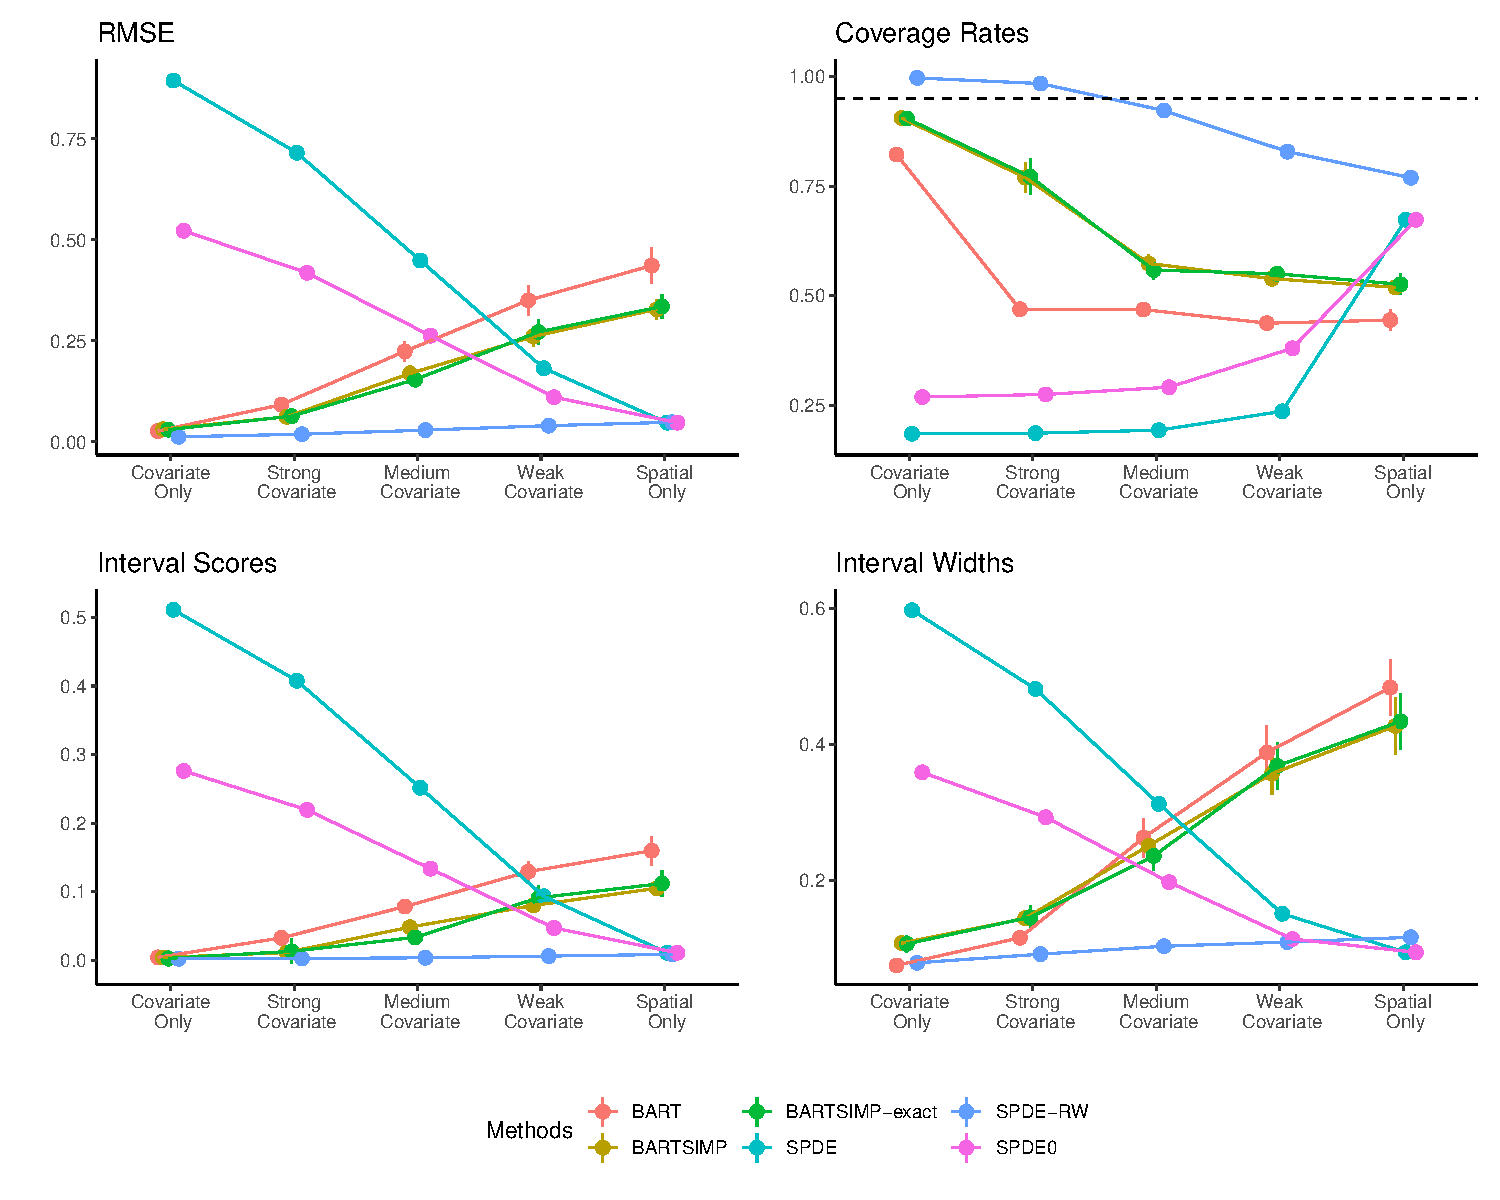
\includegraphics[width=\linewidth]{sim_study/sim_compare_smooth2.pdf}
    \caption{Root mean squared error (RMSE), average coverage rate (ACR), average interval length (AIL) and average interval score (AIS) for five different methods under five scenarios (covariate only, strong, medium, weak covariate signals and spatial signals only), when the covariate surface has a \textbf{smooth structure}. The dots show the average values over 10 replications, and the vertical lines illustrate the 95\% Wald type interval computed from the standard deviation over 10 replications. The dashed horizontal line represents the nominal coverage rate (0.95). The horizontal dashed line in the upper right figure illustrates the 95\% nominal coverage.}
    \label{fig:modcomp_smooth}
\end{figure}


\newpage

\section{Posterior Convergence Checks}

We look at the posterior convergence for the following quantities:

\begin{itemize}
    \item $\sigma_m^2, \sigma^2$ and $\kappa$: the spatial hyperparameters
    \item $\sum_{j=1}^m g(\boldsymbol{x}_{i} ; \mathbf{T}_j, \boldsymbol{\mu}_j), i \in \{400, 500, 750\}$: the fitted covariate values for the 400, 500 and 750-th row in the dataset. We refer to them as `location 1',  `location 2' and `location 3'. 
\end{itemize}

Figures 15 to 17 in Supplementary Materials, Section 9 show line plots of the 2001st-4000th posterior samples. Table 6 shows the efficient sample sizes obtained from the 2000 samples. 

\newpage

\begin{figure}[H]
    \centering
    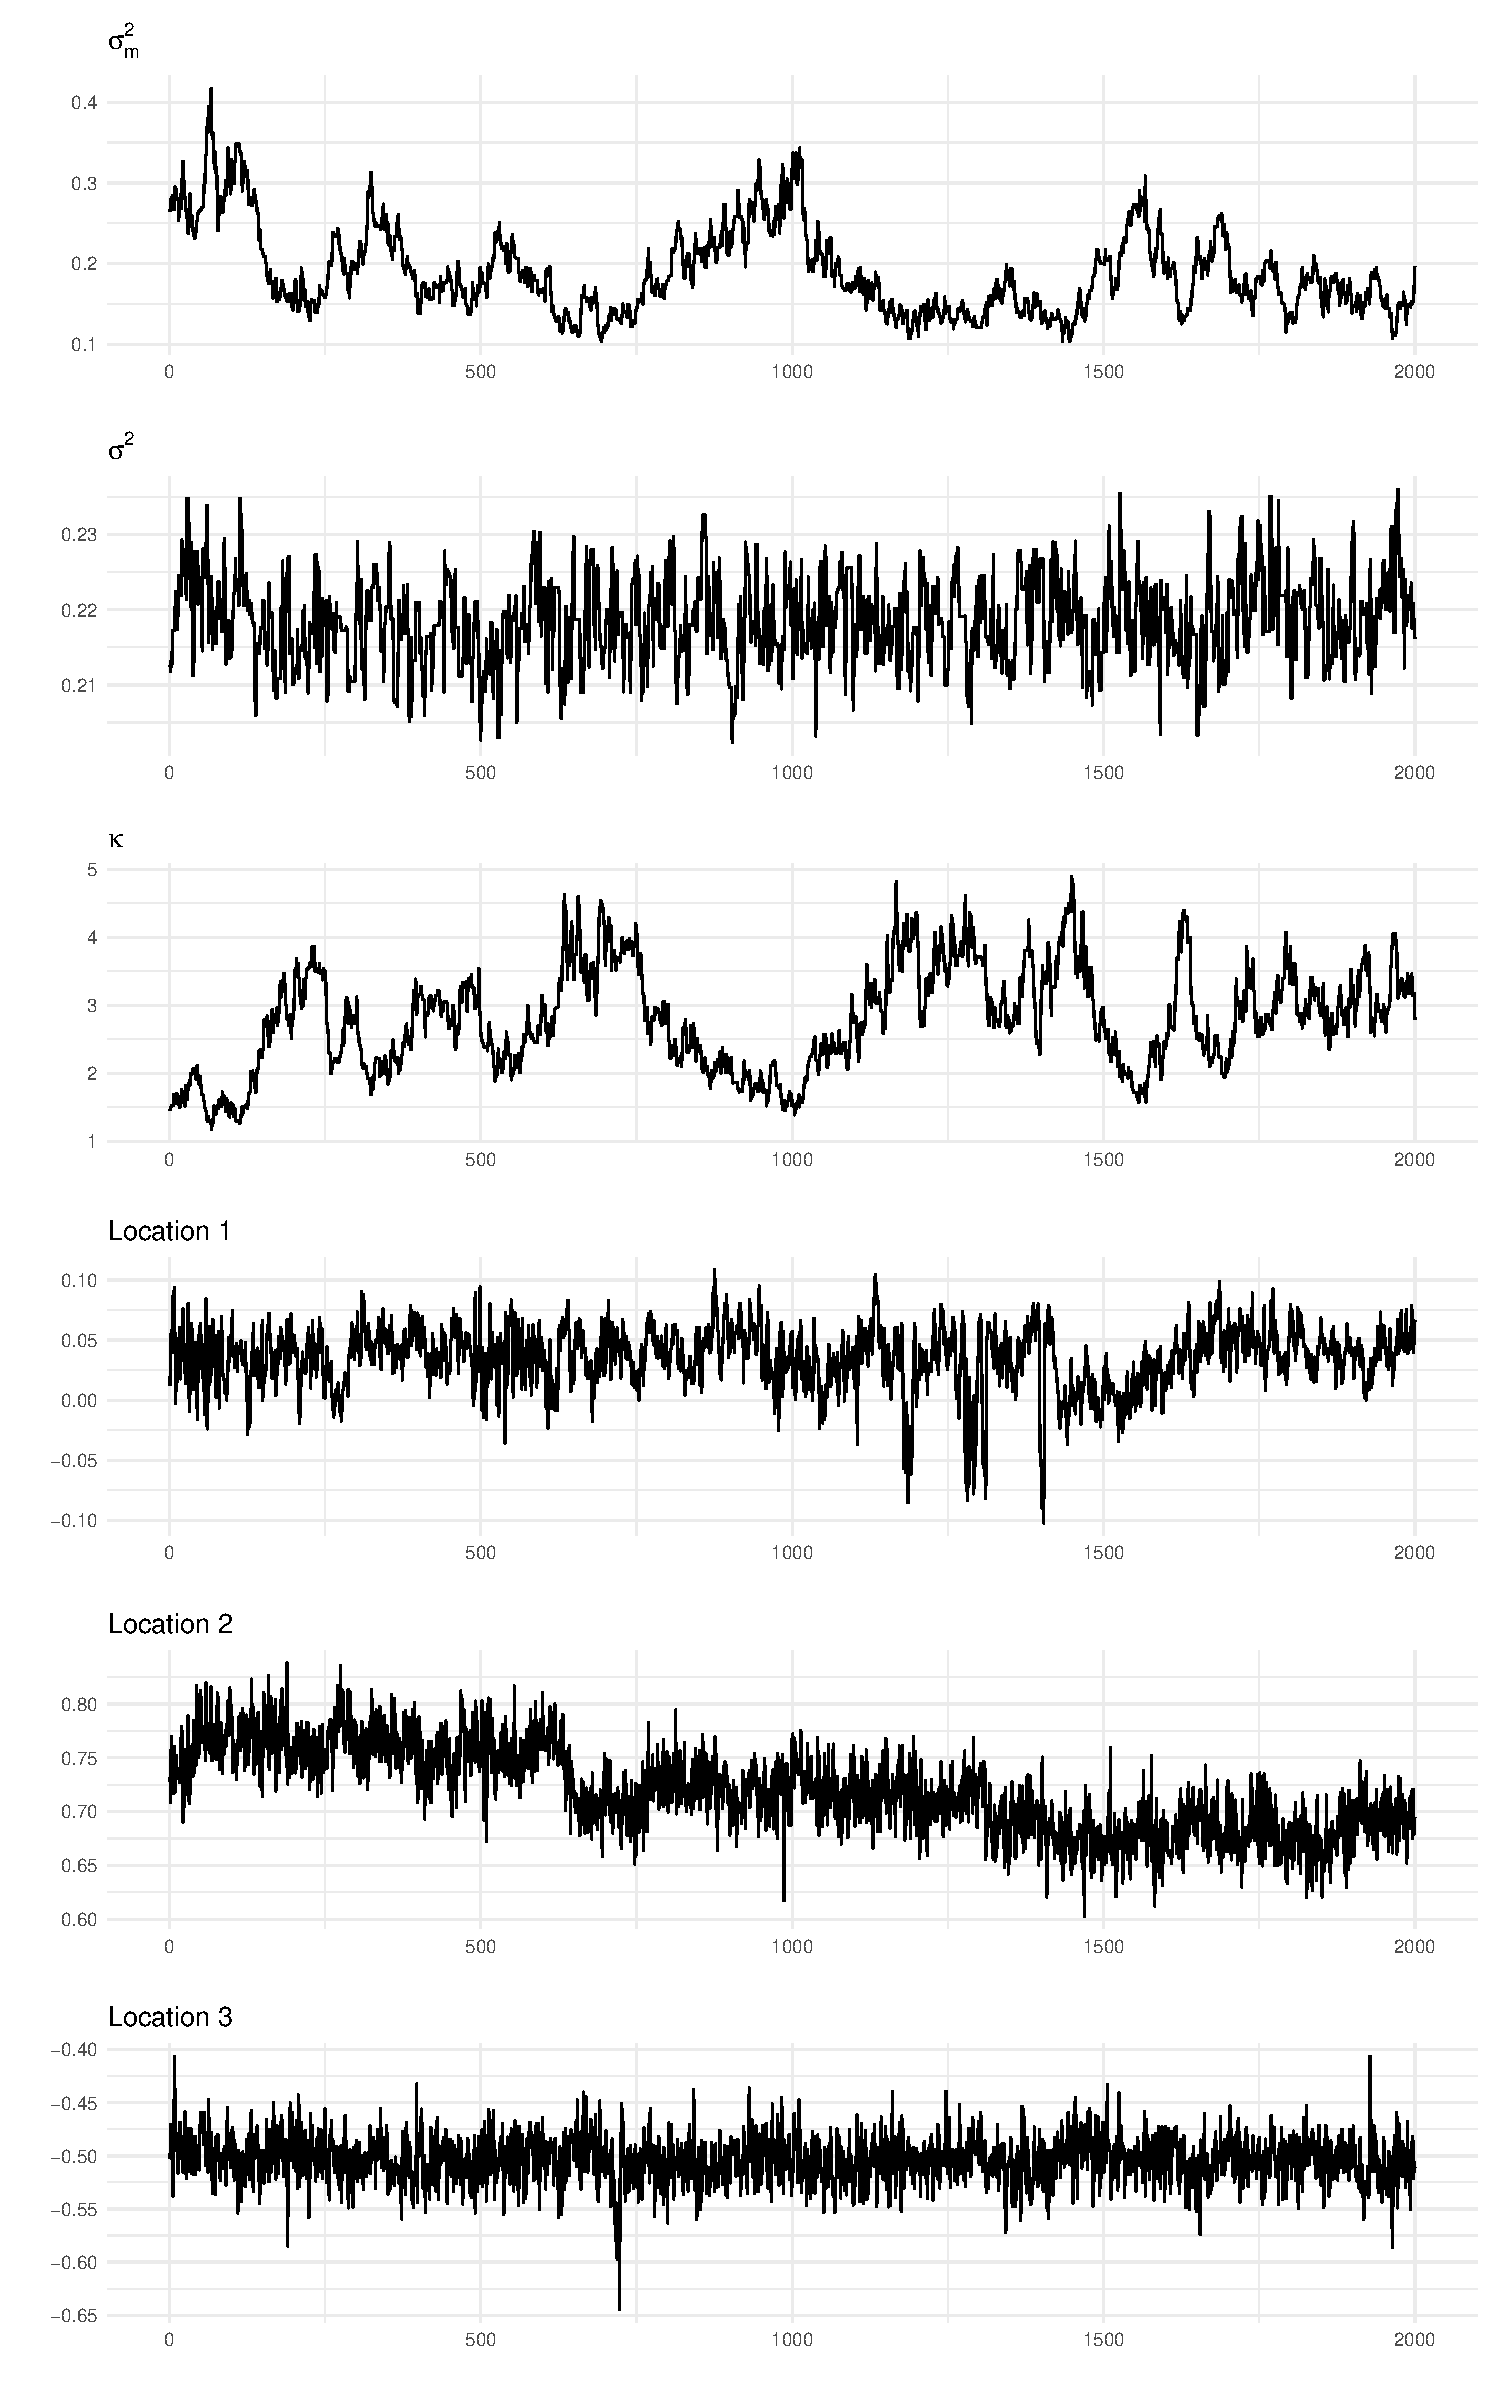
\includegraphics[width=0.8\linewidth]{convergence/mixing_data_3_scenario_3.pdf}
    \caption{Line plots for the six quantities obtained from the 2001-4000 posterior samples in dataset 1.}
    \label{fig:enter-label}
\end{figure}

\begin{figure}[H]
    \centering
    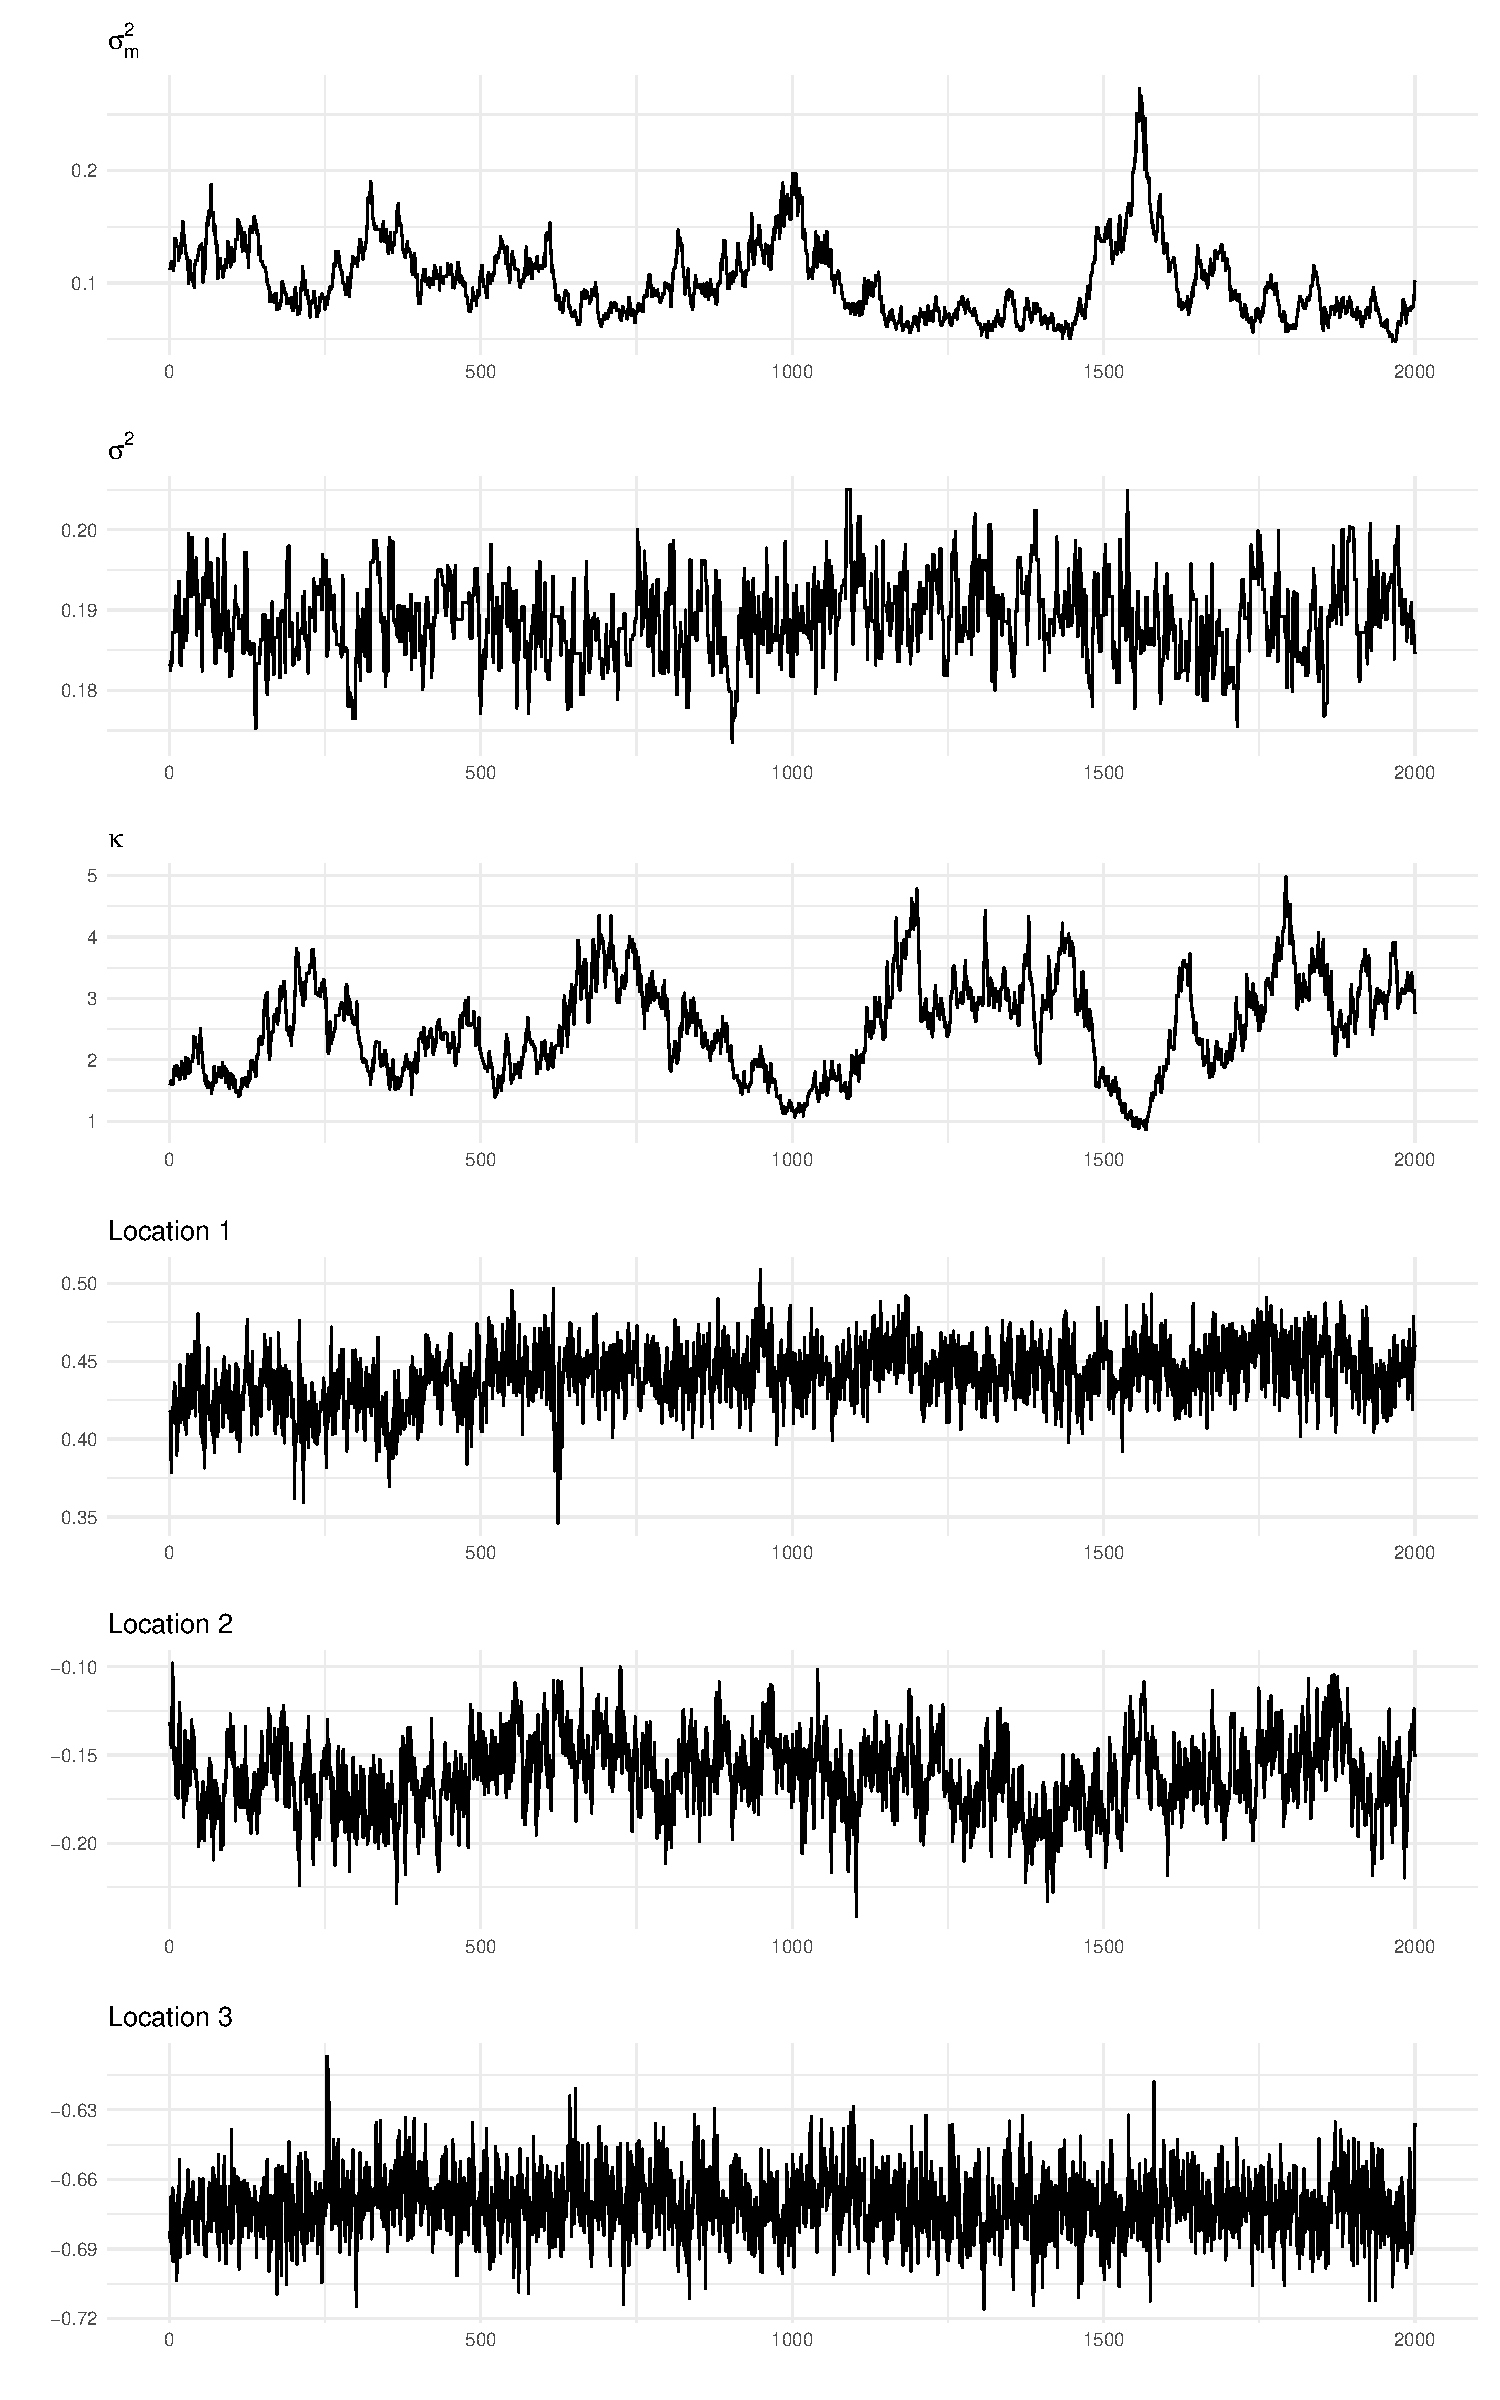
\includegraphics[width=0.8\linewidth]{convergence/mixing_data_5_scenario_12.pdf}
    \caption{Line plots for the six quantites obtained from the 2001-4000 posterior samples in dataset 2.}
    \label{fig:enter-label}
\end{figure}


\begin{figure}[H]
    \centering
    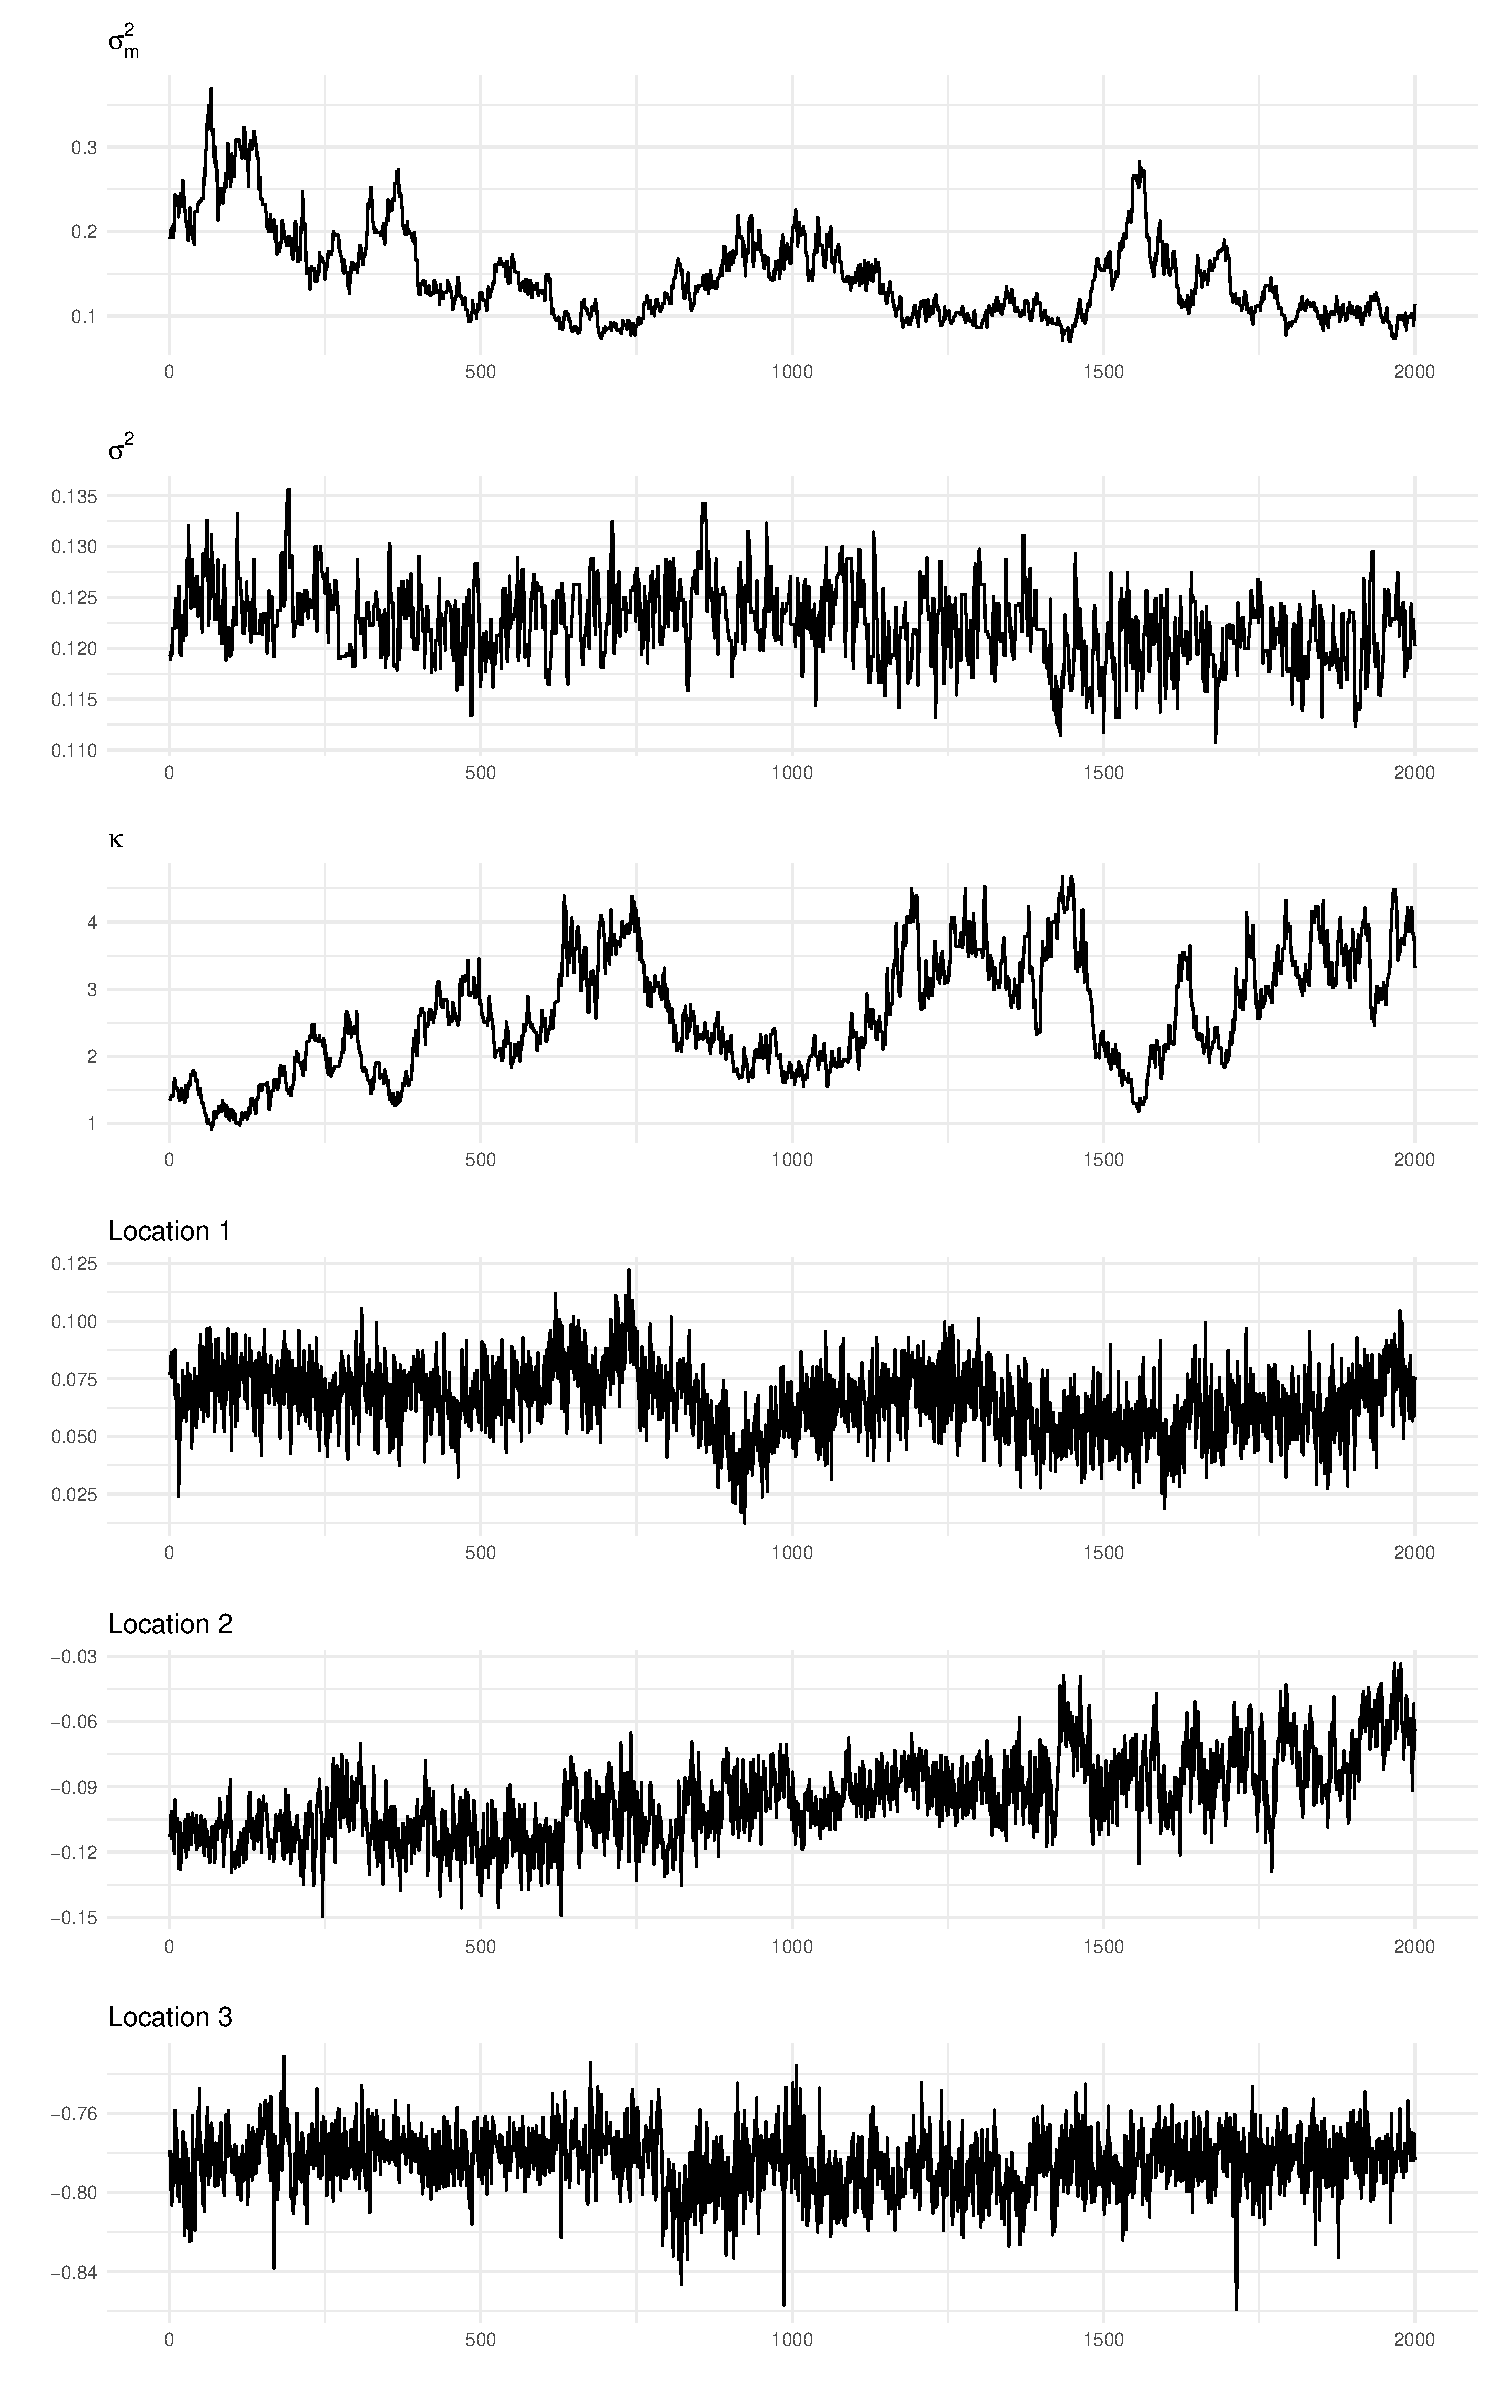
\includegraphics[width=0.8\linewidth]{convergence/mixing_data_8_scenario_7.pdf}
    \caption{Line plots for the six quantites obtained from the 2001-4000 posterior samples in dataset 3.}
    \label{fig:enter-label}
\end{figure}


\begin{table}[H]
\label{tab:conv}
\centering
\begin{tabular}{rrrrrrr}
  \hline
scenarios & $\sigma_m^2$ & $\sigma_e^2$ & $\kappa$ & $\sum_{j=1}^m g\left(\boldsymbol{x}_{400} ; \mathbf{T}_j, \boldsymbol{\mu}_j\right)$ & $\sum_{j=1}^m g\left(\boldsymbol{x}_{500} ; \mathbf{T}_j, \boldsymbol{\mu}_j\right)$ & $\sum_{j=1}^m g\left(\boldsymbol{x}_{750} ; \mathbf{T}_j, \boldsymbol{\mu}_j\right)$ \\ 
  \hline
1 & 4.94 & 380.26 & 14.68 & 476.93 & 355.51 & 854.33 \\ 
  2 & 12.44 & 262.06 & 16.79 & 152.80 & 63.37 & 168.93 \\ 
  3 & 17.74 & 303.88 & 22.52 & 79.34 & 168.82 & 176.20 \\ 
  4 & 20.21 & 298.31 & 28.15 & 54.03 & 65.46 & 148.07 \\ 
  5 & 22.46 & 332.86 & 30.10 & 64.84 & 156.82 & 173.77 \\ 
  6 & 5.07 & 307.26 & 14.51 & 136.44 & 151.67 & 414.23 \\ 
  7 & 12.61 & 254.22 & 16.13 & 100.25 & 128.84 & 127.22 \\ 
  8 & 15.87 & 305.55 & 22.00 & 87.83 & 100.86 & 293.35 \\ 
  9 & 17.01 & 314.94 & 25.09 & 130.24 & 68.70 & 128.08 \\ 
  10 & 22.46 & 332.86 & 30.10 & 64.84 & 156.82 & 173.77 \\ 
  11 & 5.27 & 204.71 & 14.90 & 109.08 & 101.36 & 312.14 \\ 
  12 & 13.04 & 246.62 & 16.13 & 102.05 & 115.11 & 365.53 \\ 
  13 & 16.31 & 300.75 & 22.27 & 79.89 & 111.96 & 69.95 \\ 
  14 & 20.78 & 324.56 & 26.43 & 100.54 & 73.72 & 157.05 \\ 
  15 & 22.46 & 332.86 & 30.10 & 64.84 & 156.82 & 173.77 \\ 
   \hline
\end{tabular}
\caption{Efficient sample sizes of the quantities of interest, averaged over 10 datasets for each scenario. Each row represents a different scenario (1-5 for `tree structured', 6-10 for `linear' and 11-15 for `smooth').}
\end{table}

\section{Details on the BARTSIMP-exact}

Consider a simple multivariate Gaussian model with zero mean and Matern covariance matrix:

\begin{align*}
    \boldsymbol{y} \mid \sigma_e^2, \sigma_m^2, \kappa \sim \mathcal{N}(\mathbf{0}, \mathbf{\Sigma} + \sigma_e^2 \mathbf{I}),
\end{align*}
where 
\begin{align*}
    \Sigma_{ij}=\sigma_m^2 \frac{2^{1-\nu}}{\Gamma(\nu)}\left(\kappa{d_{ij}}\right)^\nu K_\nu\left( \kappa{d_{ij}}\right).
\end{align*}
here, we let $\nu = 1, \sigma_e^2= \sigma_m^2 = 4, \kappa = 2$. Let $n$ be the number of observations in $\boldsymbol{y}$, the marginal likelihood has form 
\begin{align}
\label{eq:ex}
    -\frac{n}{2}\log(2\pi) - \frac{1}{2}\log \det (\mathbf{\Sigma}+\sigma_{\varepsilon}^2 \mathbf{I}) - \frac{1}{2}\boldsymbol{y}^T (\mathbf{\Sigma}+\sigma_{\varepsilon}^2 \mathbf{I})^{-1}\boldsymbol{y}.
\end{align}
The method `exact' will evaluate \eqref{eq:ex} directly. The formula can also be approximate using SPDE where the dense covariance matrix is approximated with the inverse of a sparse precision matrix, (this is implemented by INLA). Table shows the averages and standard deviations (over 10 replications) of algorithm running times for both two methods, under values $n$ 100, 500, 1000 and 5000:

\begin{table}[H]
\centering
\begin{tabular}{@{}lcccc@{}}
\toprule
 &
  $n=100$ &
  $n=500$ &
  $n=1000$ &
  $n=5000$ \\ \midrule
INLA-SPDE (BARTSIMP) &
  \begin{tabular}[c]{@{}c@{}}2.897\\ (0.334)\end{tabular} &
  \begin{tabular}[c]{@{}c@{}}3.223\\ (0.201)\end{tabular} &
  \begin{tabular}[c]{@{}c@{}}3.356\\ (0.164)\end{tabular} &
  \begin{tabular}[c]{@{}c@{}}3.453\\ (0.523)\end{tabular} 
   \\
Exact (BARTSIMP-exact) &
  \begin{tabular}[c]{@{}c@{}}0.022\\ (0.004)\end{tabular} &
  \begin{tabular}[c]{@{}c@{}}0.201\\ (0.025)\end{tabular} &
  \begin{tabular}[c]{@{}c@{}}1.725\\ (0.199)\end{tabular} &
  \begin{tabular}[c]{@{}c@{}}183.9\\ (1.980)\end{tabular} 
   \\ \bottomrule
\end{tabular}
\label{tab:my-table}

\caption{Comparison between INLA-SPDE and the exact method under different number of observations.}
\end{table}




\section{Comparison on computation time under different methods}
\subsection{Simulation Studies}

\begin{table}[H]
\centering
\begin{tabular}{lll}
\toprule
Methods & Average (min) & Standard Deviation (min)\\
\midrule
BART & 13.7 & 0.4\\
BARTSIMP & 956.4 & 261.7\\
BARTSIMP-exact & 608.2 & 314.6\\
SPDE & 4.9 & 7.1\\
SPDE0 & 5.9 & 9.6\\
SPDE-RW & 6.4 & 10.3\\
\bottomrule
\end{tabular}
\caption{Comparison of the computation time in the simulation study (with average and standard deviation over 10 datasets in 5 scenarios) among the six different methods. The numbers are shown in minutes.}
\end{table}

\subsection{Application Examples}

\begin{table}[H]
\centering
\begin{tabular}{rrrrrr}
  \hline
datasets & BARTSIMP & BART & SPDE & SPDE0 \\ 
  \hline
 1 & 520.08 & 7.73 & 0.51 & 0.48 \\ 
   2 & 510.90 & 5.36 & 0.45 & 0.53 \\ 
  3 & 515.22 & 5.15 & 0.48 & 0.51 \\ 
   4 & 513.30 & 5.00 & 0.54 & 0.52 \\ 
   5 & 515.84 & 5.18 & 0.47 & 0.50 \\ 
  6 & 481.30 & 5.12 & 0.49 & 0.48 \\ 
 7 & 483.38 & 5.17 & 0.47 & 0.46 \\ 
    8 & 449.94 & 4.55 & 0.49 & 0.52 \\ 
   9 & 427.91 & 4.78 & 0.46 & 0.58 \\ 
  10 & 426.24 & 5.25 & 0.49 & 0.40 \\ 
   \hline
\end{tabular}
\caption{Comparison of the computation time in the application example on 10 datasets among the four different methods. The numbers are shown in minutes.}
\end{table}




\end{document}

\section{Probability induced by the tree structure $T$}
\subsection{Explicit formula for $p(T)$}
In Section 3.4, we outlined the prior distribution for the tree structure variable. Here, we give an explicit expression for the prior with a numerical example in the next section. 
\begin{proposition}
Let $T$ be a decision tree, defined as in Section 3.4. Let $D$ be the depth of $T$, $\ell_n^d, \ell_t^d,  d = 0, \dots, D$ respectively be the non-terminal and terminal nodes at depth $d$ in $T$. Assuming that the numeric values in each of the variables $\boldsymbol{x}_1, \dots, \boldsymbol{x}_p$ are distinct. The prior distribution of $T$ has the following formula:
\begin{align*}
    p(T) = \prod_{d = 0}^D \left[\alpha (1 + d)^{-\beta} \right]^{\ell_n^d}\left[1 -\alpha (1 + d)^{-\beta} \right]^{\ell_t^d}\left(\frac{1}{pd}\right)^{\sum_{d=0}^D \ell_n^d}.
\end{align*}
\end{proposition}
\begin{proof} We follow the prior specification outlined in Section 3.4. First, the probability for the nodes, $P_1$, has the following formula:
\begin{align*}
    P_1 = \prod_{d = 0}^D \left[\alpha (1 + d)^{-\beta} \right]^{\ell_n^d}\left[1 -\alpha (1 + d)^{-\beta} \right]^{\ell_t^d}.
\end{align*}
The probability for the splitting variables, $P_2$ and the probability for the splitting values, $P_3$ have the following formula:
\begin{align*}
    P_2 = \left(\frac{1}{p}\right)^{\sum_{d=0}^D \ell_n^d}, && P_3 = \prod_{d=0}\left(\frac{1}{n}\right)^{\sum_{d=0}^D \ell_n^d}.
\end{align*}
Thus we have 
\begin{align*}
    p(T) = P_1P_2P_3.
\end{align*}
\end{proof}
Note that we assume that the numeric values in the variables are distinct, which is a reasonable assumption for continuous variables. For scenarios where there are ties in the numeric values from a splitting variable, the probability that a value is chosen as the splitting value is proportional to its frequency in such variable. 
\subsection{A numerical exapmle}
We consider the example where $n = 5, p = 2$; Specifically, $\boldsymbol{x}_1 = (-1, 1, 0, 2, 5)^\intercal, \boldsymbol{x}_2 = (2, -1, 0, 2, 5)^\intercal$. We let $T$ be the binary tree structure. 
Nodes 1 (at depth 0) and 3 (at depth 1) are non-terminal and nodes 2 (at depth 1), 4 and 5 (both at depth 2) are terminal, thus, we have 
\begin{align*}
    P_1 = \alpha^2(1 + 1)^{-\beta} \cdot (1 - \alpha(1 + 1)^{-\beta}) \cdot (1 - \alpha (1 + 2)^{-\beta})^2.
\end{align*}
For the non-terminal nodes, the splitting variables are randomly chosen from $\boldsymbol{x}_1$ and $\boldsymbol{x}_2$, and the splitting values are randomly chosen from the numerical values in $\boldsymbol{x}_1$ and $\boldsymbol{x}_2$. Thus 
\begin{align*}
    P_2 = \left(\frac{1}{2}\right)^2, && P_3 = \left(\frac{1}{5}\right)^2.
\end{align*}
Thus we have $p(T) = P_1 P_2 P_3$.


\bibliographystyle{apalike}
\bibliography{main}




\section{Scalability test}


\section{Introduction}

Consider a simple multivariate Gaussian model with zero mean and Matern covariance matrix:

\begin{align*}
    \boldsymbol{y} \mid \sigma_e^2, \sigma_m^2, \kappa \sim \mathcal{N}(\mathbf{0}, \mathbf{\Sigma} + \sigma_e^2 \mathbf{I}),
\end{align*}
where 
\begin{align*}
    \Sigma_{ij}=\sigma_m^2 \frac{2^{1-\nu}}{\Gamma(\nu)}\left(\kappa{d_{ij}}\right)^\nu K_\nu\left( \kappa{d_{ij}}\right).
\end{align*}
here, we let $\nu = 1, \sigma_e^2= \sigma_m^2 = 4, \kappa = 2$. Let $n$ be the number of observations in $\boldsymbol{y}$, the marginal likelihood has form 
\begin{align}
\label{eq:ex}
    -\frac{n}{2}\log(2\pi) - \frac{1}{2}\log \det (\mathbf{\Sigma}+\sigma_{\varepsilon}^2 \mathbf{I}) - \frac{1}{2}\boldsymbol{y}^T (\mathbf{\Sigma}+\sigma_{\varepsilon}^2 \mathbf{I})^{-1}\boldsymbol{y}.
\end{align}
The method `exact' will evaluate \eqref{eq:ex} directly. The formula can also be approximate using SPDE, which is implemented by INLA. Table shows the averages and standard deviations (over 10 replications) of algorithm running times for both two methods, under values $n$ 100, 500, 1000 and 5000:

\begin{table}[htb]
\centering
\begin{tabular}{@{}ccccc@{}}
\toprule
 &
  $n=100$ &
  $n=500$ &
  $n=1000$ &
  $n=5000$ \\ \midrule
INLA-SPDE &
  \begin{tabular}[c]{@{}c@{}}2.897\\ (0.334)\end{tabular} &
  \begin{tabular}[c]{@{}c@{}}3.223\\ (0.201)\end{tabular} &
  \begin{tabular}[c]{@{}c@{}}3.356\\ (0.164)\end{tabular} &
  \begin{tabular}[c]{@{}c@{}}3.453\\ (0.523)\end{tabular} 
   \\
exact &
  \begin{tabular}[c]{@{}c@{}}0.022\\ (0.004)\end{tabular} &
  \begin{tabular}[c]{@{}c@{}}0.201\\ (0.025)\end{tabular} &
  \begin{tabular}[c]{@{}c@{}}1.725\\ (0.199)\end{tabular} &
  \begin{tabular}[c]{@{}c@{}}183.9\\ (1.980)\end{tabular} 
   \\ \bottomrule
\end{tabular}
\label{tab:my-table}
\end{table}


\section{Comparison of $\mu$-sampling using GRF or GMRF}

\begin{itemize}
    \item Original method: Compute the $N \times N$ dense covariance matrix $\mathbf{\Sigma}$, where $N$ is the number of spatial locations 
    \item Approximation method: Operate on $\mathbf{\Sigma}$ with the corresponding $\mathbf{Q}^{-1}$, where $\mathbf{Q}$ is the precision matrix of the GMRF that approximates the GP
\end{itemize}



